%
% This documentation is in German (de)
% Encoding of the filse is Latin-1.
% Umlauts are written as regular characters.


\documentclass[paper=a4,pagesize,12pt,BCOR=10mm,DIV=15,headinclude=true]{scrbook}
\usepackage[german]{babel}

\usepackage[latin1]{inputenc}
\usepackage[T1]{fontenc}
%\usepackage{lmodern}
\usepackage{ae,aecompl}
\usepackage{microtype}

\usepackage{scrpage2}
\usepackage{graphicx}
\usepackage{wrapfig}
\usepackage{mdwlist}
\usepackage{array} 
\usepackage{calc}
\usepackage{fancyvrb}
\usepackage{xifthen}
\usepackage{etoolbox}
\usepackage[linktoc=page,colorlinks=true,linkcolor=black]{hyperref}
\usepackage{epstopdf}
\usepackage{xspace}
\usepackage{csquotes}

\hypersetup{
	linktoc=page,
	colorlinks=true,
	linkcolor=black,
	urlcolor=black,
	pdfauthor={Matthias Reichl} {Peter Dell},
	pdfkeywords={Atari} {8bit} {Freezer} {TURBO FREEZER} {Hardware}
}

\setcounter{secnumdepth}{3}
\setcounter{tocdepth}{2}

%\renewcommand{\ttdefault}{pcr}

%\setlength{\headheight}{1.1\baselineskip}


% Common
\newcommand{\frz}{\mbox{TURBO FREEZER}\xspace}
\newcommand{\frzs}{\mbox{TURBO FREEZERs}\xspace}
\newcommand{\zB}{\mbox{z.\,B.}\xspace}
\newcommand{\ie}{\mbox{i.\,e.}\xspace}
\newcommand{\eg}{\mbox{e.\,g.}\xspace}


% format commands and keys
\newcommand{\fcmd}[1]{\mbox{\ttfamily#1}}

\newcommand{\fpara}[1]{\mbox{\ttfamily#1}}

% switch / button
\newcommand{\fsw}[1]{\fq{\mbox{\textbf{#1}}}}

% value / setting
\newcommand{\fval}[1]{{\ttfamily #1}}

% screen message
\newcommand{\fmsg}[1]{{\ttfamily #1}}

% quote a text
\newcommand{\fq}[1]{\enquote{#1}}

% register
\newcommand{\freg}[1]{{\ttfamily #1}}

% hex number
\newcommand{\fhex}[1]{\$#1}
% hex number range
\newcommand{\fhexr}[2]{\fhex{#1}\dots\fhex{#2}}
% decimal number range
\newcommand{\fdecr}[2]{{#1}\dots{#2}}

% keys: with brackets
\newcommand{\fkey}[1]{\mbox{\ttfamily[#1]}}
% SHIFT+key
\newcommand{\fkeys}[1]{%
  {\ttfamily [Shift]%
  \ifthenelse{\isempty{#1}}{}{$+$[#1]}%
  }%
}
% CONTROL+key
\newcommand{\fkeyc}[1]{%
  {\ttfamily [Control]%
  \ifthenelse{\isempty{#1}}{}{$+$[#1]}%
  }%
}

% source code
\DefineVerbatimEnvironment{fcode}{Verbatim}{xleftmargin=10mm,formatcom=\setlength{\topsep}{0cm}}

% environment for manpage-style lists
\newlength{\fitemlen}
\newcommand{\fentrylabel}[1]{%
 \settowidth{\fitemlen}{#1}%
 \ifthenelse{\lengthtest{\fitemlen > \labelwidth}}%
  {\parbox[b]{\labelwidth}%
   {\makebox[0pt][l]{#1}\\}}%
  {#1}%
 \hfil\relax%
}

\newcommand{\flistlength}[1][\empty]{%
 \ifthenelse{\equal{#1}{\empty}}%
   {\setlength{\labelwidth}{4.5em}}%
   {\setlength{\labelwidth}{#1}}%
 \setlength{\parsep}{0cm}%
 \setlength{\leftmargin}{\labelwidth+\labelsep}%
}

% standard list
\newenvironment{flist}
 {%
  \begin{list}{}{%
   \flistlength%
   \renewcommand{\makelabel}[1]{\fentrylabel{##1}}%
  }%
 }%
 {\end{list}}

% nested list, smaller labelwidth and no topsep
\newenvironment{flistn}
 {%
  \begin{list}{}{%
   \setlength{\topsep}{0cm}%
   \flistlength[1.5em]%
   \renewcommand{\makelabel}[1]{\fentrylabel{##1}}%
  }%
 }%
 {\end{list}}

% command lists
\newenvironment{fcmdlist}
 {%
  \begin{list}{}{%
   \flistlength%
   \renewcommand{\makelabel}[1]{\fentrylabel{\fcmd{##1}}}%
  }%
 }%
 {\end{list}}

\newenvironment{fcmdlistn}
 {%
  \begin{list}{}{%
   \setlength{\topsep}{0cm}%
   \flistlength[1.5em]%
   \renewcommand{\makelabel}[1]{\fentrylabel{\fcmd{##1}}}%
  }%
 }%
 {\end{list}}

\newenvironment{fvallist}
 {%
  \begin{list}{}{%
   \flistlength%
   \renewcommand{\makelabel}[1]{\fentrylabel{\fval{##1}}}%
  }%
 }%
 {\end{list}}

\newenvironment{fvallistn}
 {%
  \begin{list}{}{%
   \setlength{\topsep}{0cm}%
   \flistlength[1.5em]%
   \renewcommand{\makelabel}[1]{\fentrylabel{\fval{##1}}}%
  }%
 }%
 {\end{list}}

\newenvironment{fmsglist}
 {%
  \begin{list}{}{%
   \flistlength%
   \renewcommand{\makelabel}[1]{\fentrylabel{\fmsg{##1}}}%
  }%
 }%
 {\end{list}}

\newenvironment{fmsglistn}
 {%
  \begin{list}{}{%
   \setlength{\topsep}{0cm}%
   \flistlength[1.5em]%
   \renewcommand{\makelabel}[1]{\fentrylabel{\fmsg{##1}}}%
  }%
 }%
 {\end{list}}

% memory range list
\newenvironment{fmemlist}
 {%
  \begin{list}{}{%
   \flistlength[7em]%
   \renewcommand{\makelabel}[1]{\fentrylabel{##1}}%
  }%
 }%
 {\end{list}}


\newlength{\fbitwidth}

\newcommand{\fadef}[3]{{#1}: {#2} ({#3})}

% address / byte definition: address, name, r/w
\newenvironment{fadrdef}[3]
  {\setlength{\fbitwidth}{\linewidth/8-\tabcolsep*2-\arrayrulewidth*9/8}%
    \vspace{2ex}
    \textbf{{#1}: {#2} ({#3})}%
    \par\noindent%
    \begin{tabular*}{\linewidth}%
      {*{8}{|>{\centering\hspace{0pt}}p{\the\fbitwidth}}|}
      \hline
      7 & 6 & 5 & 4 & 3 & 2 & 1 & 0 \tabularnewline
      \hline
  }
  {\tabularnewline \hline \end{tabular*}\par \vspace{0.5ex}}


\hypersetup{
	pdftitle={TURBO FREEZER XL/XE 2011 Anleitung}
}
\begin{document}

\overfullrule=2mm

\pagestyle{scrheadings}
\setheadsepline{.2pt}

\begin{titlepage}
\thispagestyle{empty}
\begin{center}
\vspace*{9cm}

{\Huge\bfseries\sffamily TURBO FREEZER XL/XE 2011}

\vspace{10cm}

Anleitung f�r Softwareversion 3.10\\
Letzte Aktualisierung am 27.~3.~2013

\end{center}
\end{titlepage}


\clearpage
\thispagestyle{empty}

\null
\vfill

\noindent Copyright \copyright 1987-2013 Peter Dell, Florian Dingler,
Bernhard Engl, Matthias Reichl
\newline

\noindent
This manual is protected by copyright and subject to Creative Commons license\linebreak
BY-NA-SA 3.0.\newline
\url{http://creativecommons.org/licenses/by-nc-sa/3.0/legalcode}\newline
\newline
This means you must attribute the work in the manner specified by the author or
licensor. You may not use this work respectively the licensed content for
commercial purposes. If you alter, transform, or build upon this work, you may
distribute the resulting work only under the same or similar license to this
one.

\clearpage

\tableofcontents

\chapter*{Preface}
\markboth{}{Preface}

\section*{Preface by the designer of the new freezer (2012)} \frz 2005
was a big success. It was very well received in the Atari community and we got
lots of positive feedback and ideas for new features. The decision to use a
flash ROM instead of an EPROM proved being particularly helpful. It enabled
users to enjoy software updates and new features as the flash ROM could be
updated from the Atari.

In particular the debugger has been extended considerably since the first
release 2005. An online help, commands for moving and comparing memory blocks, a
memory usage map and an OS vector overview, the possibility to log the screen
output of debugging sessions to printer in parallel and many additional things have
been added. Special thanks go to Erhard P�tz and Carsten Strotmann for many
good ideas.

The initial run sold out fairly quickly and requests for more kept coming. In
2010 things became more concrete. Together with Wolfram Fischer, who also
participated in the first run, I started planning a new production run.
Meanwhile the Lattice M4A5 CPLD had become relatively hard to get and was
clearly more expensive than comparable chips. We also wanted to use a slightly
\fq{larger} chip in order to implement some new ideas and features. So we
decided to use a Xilinx XC95144XL as the basis for the new freezer. Having about
the same price it offered more than twice the power (I/O pins and space for
logic) than the Lattice CPLD. This way we had the possibility of implementing
long-awaited features -- for example the RAM extension which had been there in
the very first freezer from 1987.

By the end of 2010 Wolfram had created the first prototype of the new hardware.
This was the basis for starting the development of the new logic and software at
the begin of 2011. I realized quickly that the best way would be to develop the
logic from scratch and to separate the functional blocks (freezer, cartridge
emulation, etc.). This simplified extensions in each functional block.

The logic of the cartridge emulation was completely  redone; the freezer logic
has intentionally been kept compatible with old \frz 2005 logic. I
wanted to keep the changes to the freezer software at a minimum, so it can also
be used with the \fq{old} freezer. This way the users of the old freezer may
also benefit from further updates.

In summer 2011, after several new hardware revisions and many changes to the
software and the logic, the new freezer was completed! Unfortunately the start
of the mass production, which had been planned for end of 2011, had to be
postponed by almost one year. Wolfram had to move to a new residence and was
busy at his job -- hence we both had almost no time left for our hobby. Thanks
to the support from the ABBUC the production finally started in autumn 2012!
Many thanks to Wolfgang Burger for the support. Also thanks to all who ordered
the new freezer in advance and waited so patiently.

\medskip Salzburg, November 2012

\medskip Matthias Reichl

\medskip P.S. (March 2013): I'd like to add a big \fq{thank you} to Peter Dell
who took over the job of translating the German manual into English.
At the end this was a whole lot more of work than expected, but Peter
was really brave and did an awesome job -- thanks Peter!

\section*{Preface by the designer of the new freezer (2005)} The project to
design a new \frz started in early 2004, when Bernhard Engl gave
permission to the ABBUC to remake his products (The TURBO 1050 and the \frz).
To me, the \frz has always been the most interesting piece of
hardware extension that has ever been available for the Atari and before
starting the project, I had already studied and analyzed how it worked.
That's why it was pretty obvious that I would engage in rebuilding the \frz{}.
There were more participants in the team: Bernhard Pahl, Florian
Dingler, Torsten Schall, Guus Assmann, Frank Schr�der and towards the end also
Wolfram Fischer.

So I would like to express big thanks to all of you. The project wouldn't have
come this far without you!! And some special thanks to Guus, for the many ideas
for extensions, designing the PCBs and producing the prototypes. Thanks as well
to Bernhard Engl for his tips and the detailed information for the original
\frz. All other team members, thanks for the support and the testing!

My original plan was to remake the freezer, using modern parts. At this point, I
never imagined that the result would be such extensive and powerful
improvements! During the project, both hardware and software have been gradually
extended and improved up to a point where only the basic (and genius) principle
idea of the freezer was left. Everything else had been changed.

Some of the extensions came by as pure coincidence. For example the cartridge
emulation: As 16K EPROMs were much more expensive, Guus suggested using a flash
ROM. To enable programming this flash ROM from the Atari, it was needed to map
the chip into the memory-map of the Atari.
This formed the basis for the cartridge emulation :-)

Likewise with the RAM: The original 2K RAM was hard to get and also quite
expensive. So the first step was to upgrade to a 32K chip and also use 128K
flash ROM. The next step was to go to 128K RAM and this made it possible to put
a memory-snapshot into this RAM. And the flash ROM size was increased to 512K.
To enable this, the logic had to be improved. And a bigger logic chip gave space
for the emulation of the 16K OSS modules and the SpartaDOS~X module.

With the current state of the logic chip's internals, there's no space left and
we're all content to have gotten the maximum out of the parts that were used.
For the software, there are some more ideas for extensions, but that's all I'll
say for now.

During the development process, I've constantly kept in mind that I wanted to
create an open basis for further developments. For this reason, all design
information is freely available and there's even a JTAG interface on board
so the logic can be reprogrammed. This will help anyone who wants to expand the
freezer or even make something completely new with it.

All relevant information and updates for the \frz XL/XE 2005 are
available on the internet at \url{http://turbofreezer.horus.com/}. There's also
a manual on how to alter the logic of the \frz. For technical
questions, write an e-mail to
\href{mailto:hias@horus.com}{\nolinkurl{hias@horus.com}}.

The many features of the \frz have not only convinced the team
members, but also many members of the ABBUC. In their Hardware Contest 2005, it
was awarded a very convincing first prize.

I wish you a lot of fun using the \frz and stay loyal to the Atari
8-bit computers for many years to come.

\medskip Salzburg, December 2005

\medskip Matthias Reichl.

\section*{Preface by the developer of the original freezer (2005)} As a
designer, the best recognition of achievement one can get, is that a once
successful product is continued and enhanced by a competent successor. However,
if this happens after 16 years and for a home-computer product, it's downright
sensational and means that the product has attained cult status. While using
original concept of the 1980's, Matthias Reichl has made a real masterpiece of
the \frz XL/XE 2005. The application of modern micro-chips has led to
a great extension of the functionality. He even managed to remove some minor
bugs that were known, but couldn't be prevented using the electronics of that
time, without making the product economically impossible because of the higher
chip-count.

The improvements and enhancement, especially the ingenious cartridge emulation
that was not present in the original, make the \frz XL/XE not only
the best and most perfect freezer for the 8-bit Atari that ever existed, but
also is an all-rounder talent, having the potential to become a legendary cult
product. At this point in time, it's a high-light of a technical development
that started more than 20 years ago. In my notebook, which has turned yellow
now, the first sketches of the concept date back to the autumn of 1984. Finding
this out even surprised myself.

Experiencing a vastly improved, enhanced and rejuvenated new series of a
computer extension product, is not only a miracle, but also a special joy and
honor to me, so I wish all proud owners of the new \frz XL/XE a lot of
pleasure using it.

\medskip Zurich, November 2005

\medskip Bernhard Engl

\section*{Preface by the developer of the original freezer (1987)}
After one year development, hundreds of used-up integrated circuits, 5300 lines
of assembler code and five-digit costs, it's there at last:
The \frz XL. It's not only the first real freezer for the Atari, it is
also the only extension a freak needs to get the optimum and maximum usage out
of his Atari. This is because apart from freezer, the board also offers a socket
for an Oldrunner and for 256k of RAM so an 800 XL can be extended to up to 320k.

By using three ASICs containing the equivalent of over 40 TTL circuits and by
avoiding a costly multi-layer PCB, all this could be implemented at an unbeatable
price. In addition, thanks to the very powerful memory management that is anyway
needed for the freezer, the computer doesn't need to be opened.

The careful same tuning of all components can be found in the built-in software
which consists of the freezer, a mini-DOS and a debugger. Combined with the
hardware, this power-tool gives an unprecedented possibility of control over
programs to the user. That's why anyone who's seen the \frz XL in
action, wanted to have one as well. The thrill of having total control over the
computer, even though the programmer did not want this, is well worth the price.
And then there's also the money save from buying separate extensions that would be
needed to get the same functions that are present in the \frz XL.

More about this in the description of the individual functions! I wish every
proud owner lots of fun with the most fascinating product that was ever
available for the Atari.

\medskip Munich, May 1987

\medskip Bernhard Engl

\chapter{Installation}

The \frz is simply attached to the parallel bus. The parallel bus differs
between Atari XL and XE computers. In Atari XL computers the parallel bus
consists of the Parallel Bus Interface (PBI) which is labeled \fq{Parallel Bus}.
In Atari XE computers the parallel bus consists of the cartridge port and the
Enhanced Cartridge Interface (ECI) which are labeled \fq{Cartridge} and
\fq{Expansion}. The power supply of the \frz is taken from the parallel bus. In
Atari 600 XL and older Atari 800 XL computers the required power is available
directly on the parallel bus. It is no longer available there in new Atari 800
XL models and therefore has to be taken from the joystick port using the
power supply wire that is soldered to the freezer. Neither opening the Atari nor
soldering of any kind is required. Yet users with experience in soldering and with the
appropriate equipment have the option to add additional features.

The \frz consists of two parts, the freezer electronic in the black case and an
adapter board which establishes the connection to the PBI or ECI. The
adapter boards are available separately and hence provide a simple and cheap way
to use a \frz with Atari XL as well as with Atari XE computers.

\begin{figure}[h]
  \centering
  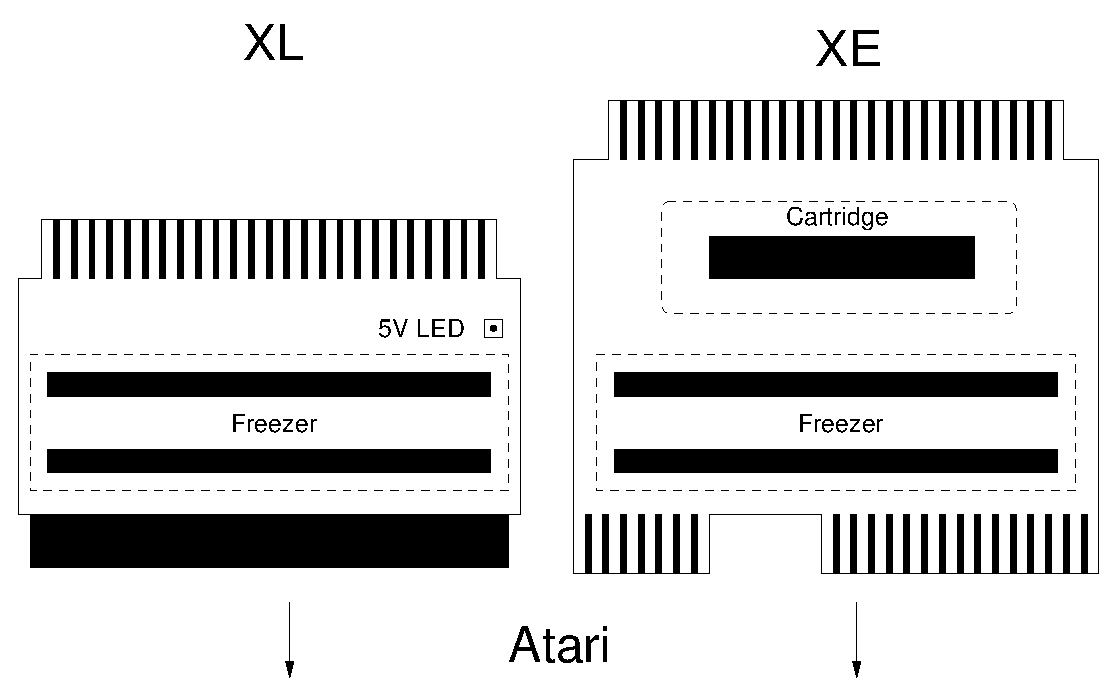
\includegraphics[width=35em]{adapter.eps}
  \caption{Atari XL and XE adapter boards}
\end{figure}

There is a small number of models from the XE series (mainly 65 XE) which do not
have an ECI port. These models only have a \fq{Cartridge} port and have no
\fq{Expansion} port. The freezer can unfortunately not be used with these XE
models. \newline

\textbf{Caution:} The freezer electronic and the adapter board are not connected
when they are shipped to prevent damage during transport. The Atari should
always be switched off to also prevent damage when attaching or detaching the
adapter board to/from the Atari or when attaching or detaching the freezer
electronic module to/from the adapter board.

\section{Verifying the power supply}
\label{sec:pbi5v}

Owners of Atari XL computer should verify the availability of the 5V power
supply on the PBI before assembling the freezer. Owners of Atari XE computer can
skip to the next step.

First switch the Atari off. Then attach the empty Atari XL adapter board without
the freezer electronic module to the PBI. Now switch the Atari on. If the 5V LED
on the adapter board lights up, then the 5V power supply is available on the PBI
and the power supply wire to the joystick port is not required. Even so, the
external power supply wire should not be cut off, but rolled up and put away
because it may be required for use on a different Atari without the PBI power
present. After that, switch the Atari off again and detach the adapter board
from the PBI.

\section{Assembling the freezer}

\subsection{Protecting from electro-static discharge}

You should \textbf{electrically ground} yourself before assembling the freezer
to discharge electro-static potentials which may be caused for example by the
carpet, shoes, clothing and so on. These potentials can reach several 1000 volts
and might destroy the XILINX chip and other ICs of the freezer. \textbf{Also
never touch the multi-pin connectors of the freezer without being grounded.}
This is true in general for all kinds of electronic parts. And though the Atari
is not too sensitive in this regard, it may still get damaged.

You best touch the heating or the protective earthing conductor pin of a power
outlet. Well suited, and very common in the professional area, are ESD
(electro-static discharge) wristbands to ground you permanently.

\subsection{Connecting the freezer electronic with the adapter board}

At the bottom of the module with the freezer electronic there are two multi-pin
connectors with 2x25 pins each. On the adapter board there are two female
connectors with 2x25 pins each. The freezer module with the freezer electronic
must be plugged into the adapter board in a way that the front side with the
switches points towards the PBI or ECI port of the Atari.
\textbf{The module must never be plugged in the other way around because that
may destroy the freezer.}

At first the module with  the freezer electronic must be positioned over the
female connectors in a way that all pins of the multi-pin connectors are located
over the corresponding female connectors. \textbf{No pins must overlap.} The
best way is to hold the module with the electronic in one hand and the adapter
board in the other hand.
Then place the module carefully on the board but do not press it and check from
all sides that the pins are aligned correctly. Now connect the module with the
adapter board using firm pressure. This works best if you turn the freezer
upside down. Use the fingers of both hands to hold the module on the left and
right side and then press the adapter board firmly in from the bottom with your
thumbs.

After plugging the module in you should verify that all pins are completely
inserted in the female connectors. If there are pins overlapping on one side,
the module with the freezer electronic must be unplugged and must be plugged
in again with correct alignment. If the pins are not completely inserted into
the female connectors you should firmly press until no part of the pins can be
seen anymore.

\subsection{Disconnecting the freezer electronic from the adapter board}

First the Atari must be switched off and the freezer must be detached from the
PBI or ECI port. The freezer electronic and the adapter board are quite
tightly connected via the 50 pin connectors. \textbf{You must never use too much
force or perform abrupt moves} otherwise the pins may break and the freezer can
be destroyed.

The following procedure works best: Lift the freezer module with the thumb by
pushing the left and the right edge of the freezer module in the middle between the
two multi-pin connectors. Lift it step by step carefully by $0.5$ up to at most
1 mm on one side and then on the other side. Make sure to pull out the contacts
equally on the left and right edge as well as in the front and the back row.

After about 2~mm the female connectors lose their grip. Now you have to
proceed with special precaution because otherwise the pins will be bent easily.
After about 5~mm you are done and the freezer electronic is disconnected from
the adapter board.

\section{Plugging the freezer in}

\subsection{Atari 600 XL (at least 64k RAM) and Atari 800 XL}

Remove the snapped in PBI plastic cover, bend the metal shielding carefully away
a little bit with your fingers and attach the freezer without using force.

\begin{wrapfigure}{r}{8em}
\centering\includegraphics[width=8em]{joyport.eps}
\end{wrapfigure}
If the PBI
has a 5V power supply (see section \ref{sec:pbi5v}), the connection to the
joystick port can be omitted. If the power supply is not available on the PBI,
the power supply wire must be connected to pin 7 of the joystick port 2. Pin 7
is marked in the figure on the right.\newline

\textbf{Caution:} The power supply wire must never be disconnected while the
Atari is switched on, otherwise the Atari and/or the freezer can be damaged. If
the power supply wire is disconnected accidentally, the Atari must be switched
off immediately.

\subsection{Atari 800 XE, 65 XE and 130 XE}

Attach the freezer to the cartridge port and the ECI port at the back of
the Atari.


\section{Turning the freezer on}

\subsection{Setting the basic configuration}
\label{sec:baseconfig}

Turn all freezer switches to the left to activate the following basic
configuration:
\begin{itemize*}
\item \fsw{CartEmu}: \fval{OFF}, cartridge emulation off
\item \fsw{FlashWrite}: \fval{OFF}, write enable for flash ROM off
\item \fsw{OldOS}: \fval{OFF}, Oldrunner off
\item \fsw{Stereo}: \fval{OFF}, stereo POKEY mode off (not present)
\item \fsw{Ramdisk}: \fval{OFF}, 512k RAM extension off
\end{itemize*}

\begin{figure}[h]
  \centering
  \includegraphics[width=22em]{freezer2011.eps}
  \caption{Switches on the \frz}
\end{figure}

\subsection{Activating the freezer}

Switch the Atari computer on and leave all other hardware switched off. If the
\fmsg{READY} message of the BASIC does not appear after the usual short delay,
but other suspicious symptoms occur (system crash, black screen, smoke), switch
the system off immediately and look for the problem. If the Oldrunner is active,
the message \fmsg{ATARI COMPUTER - MEMO PAD} is displayed instead of the \fmsg{READY}
message. If the cartridge emulation is active, the green screen with the
\fmsg{TURBO CARTRIDGE} menu of the cartridge emulation is displayed. In these
cases verify that you have really setup the basic configuration according to
section \ref{sec:baseconfig}.

If \fmsg{READY} is displayed, simply press the \fsw{Freeze} button on the
upper right to display the freezer main menu. If nothing happens, the freezer is
attached poorly, the power supply wire (if present) is not connected correctly
or the freezer broke down. By pressing the \fkey{SPACE} key you can return from
the freezer main menu to the BASIC. Now verify if BASIC reacts to keyboard
input. If this is not the case, then there is a problem. If everything worked
fine up to this point the freezer is ready.

If the freezer does not work correctly for any reason, send a letter or e-mail
with the description of the symptoms first before sending the freezer back.
Because of the 100\% final assembly tests of every freezer it is practically
impossible that the problem is due to the freezer. Most likely the assembly or
the Atari itself are the cause for the problem. It is better to rule out these
possible reasons before sending the freezer back for verification. This prevents
unnecessary delays and costs.

\subsection{Creating the system disk}

Right after the successful installation of the \frz a system disk should be
created. The system disk contains the flash program for writing to the flash ROM
from the Atari and the freezer software. With this disk the \frz can be reset
at any time to its state at delivery. In the state at delivery the flash ROM
contains the software required for creating the system disk as follows:

\begin{enumerate}
\item Switch the Atari off and connect a disk drive.
\item Turn the \fsw{CartEmu} switch right to activate the cartridge emulation.
\item After switching the Atari on the menu of the cartridge emulation should
appear.
\item Press \fkey{D} to load the default settings and confirm them with \fkey{RETURN}.
\item Now you are in the \fq{\frz System Disk Writer} software. Insert an empty
disk in the disk drive \fq{D1:} and press \fkey{RETURN}. The software now
formats the disk in medium density and writes the freezer software.
If an error occurs (\eg due to a disk defect), the message \fmsg{ERROR} is
displayed and you have to insert a new disk and restart the program. To this
end simply confirm the \fmsg{restart program?} prompt with \fkey{Y}.
To be on the safe side, a second copy of the system disk should be created.
Write protect this second copy and store it in a safe location.
\item After creating the system disk successfully, switch the Atari off and turn
the\linebreak
\fsw{CartEmu} switch back (to the left) again to its original position.
\end{enumerate}

If anything goes wrong and you lose the system disk or overwrite it
accidentally (yes, things like that can happen sometimes), there still is the
option to download an ATR disk image of the system disk from the internet at
\url{http://turbofreezer.horus.com}.

\subsection{Activating the stereo POKEY mode (optional)}

If the Atari has a stereo POKEY extension that is in stereo mode, the
\fsw{Stereo} switch must be turned right. This way the freezer also saves the
hardware registers of the second POKEY in the shadow RAM. When the freezer is
activated, the second POKEY is disabled. When the program is resumed, its
correct previous state is restored again.

The general rule is that the position of the switch must correspond exactly to
the configuration of the Atari. Changing the switch position during operation is
allowed, but then the shadow RAM will contain wrong information. To fix this you
have to press \fkey{RESET} to trigger a re-initialization of the custom chip
area by the operating system. Alternatively change the switch position only when the
Atari is switched off.

\subsection{Activating the integrated 512k RAM extension (optional)}

As a special feature the freezer contains an integrated, battery backed 512k RAM
extension. With this every Atari can be extended easier than ever from 64k to a
total of 576k. And since the RAM extension is battery backed, the data in the
RAM extension remains intact also after switching the Atari off.

Turning the \fsw{Ramdisk} switch right activates the RAM extension. A possibly
present internal RAM extension in the Atari is automatically deactivated then.

\subsection{Using cartridges with the Atari XE}

Because the freezer occupies the cartridge port on Atari XE computers, there is
an additional cartridge port present on the XE adapter board. With this you can
continue to use cartridges even though the freezer is attached. The cartridges
have to be plugged in the adapter board with the label towards the Atari. Never
plug the cartridge in the wrong way, otherwise the cartridge, the freezer and
the Atari can be damaged.

There are cutouts around the cartridge port where a \fq{plastic tray}, like
those that are present in the cartridge port of Atari XL computers, can be
inserted. This relieves you from the tedious unlocking some cartridges require.
These \fq{plastic trays} are unfortunately not available separately. The only
way to obtain one is taking a defective Atari XL computer apart.

\section{Extended configurations for experts in soldering}

{\bfseries Warning: All of the following extensions are definitely only for
experts in soldering. If you are not such an expert strongly consider
finding one rather than trying this yourself. It is not worth ruining the poor
Atari or the freezer due to unhandiness.}

\subsection{Providing an internal power supply}
\label{sec:add5vpbi}

Whoever owns an Atari 800 XL without power supply on the PBI can add this
retroactively, but this is difficult and requires good skills. If you are not
confident enough you can simply prolong the power supply wire of the freezer to
the power supply inside the Atari. In both cases the joystick port remains free
for its actual purpose.

To discourage beginners, the following description of the modification is
limited to the absolute minimum. Experts will get along without problems. If you
found an \fq{expert} and realize that he is groping in the dark, then this is
the last chance to stop this obvious amateur.

You can tap the power supply at the end of L1 from where a conductor path leads
to the shielded part. The ferrite bead is located within spitting distance to
the power switch. To this spot you can either solder the prolonged power supply
wire of the freezer, or use two wires to connect the 5V power to pins 47 and 48 of the PBI.
These pins are the second to last pins before pin 49 and 50. One is one the
upper side of the board, one is on the lower side of the board. Soldering to the
lower side is much more difficult because the Atari must be disassembled
completely for this. In addition soldering to the ends of the mating surface
without having solder creeping to the active part of the  mating surface is
finicky. The latter must be prevented in any case.

\subsection{Installing a SYSTEM RESET key}
\label{sec:systemreset}

For using the Oldrunner and for freezing programs which do not use interrupts,
it is beneficial to install a \fkey{SYSTEM RESET} key which triggers a
non-maskable interrupt (NMI) that cannot be disabled. The key button is
installed such that pin 6 of the ANTIC can be switched to ground. It is best to
connect the key button to the corresponding pull-up resistor. You can tap the
pin at best at the pull-up resistor. In the Atari 800 XL and all Atari XE models
this resistor is R1. In the Atari 800 XL it is R34, and in the Atari 1200 XL it
is R7.

{\bfseries Warning: In addition to the general warning from the first section it
applies here that mechanical works are required to install the key button.
These works require additional tools and manual skills to achieve a good-looking
result.}

\subsection{Providing compatibility with 1MB RAM extensions}

The \frz uses the refresh line to stop the Atari. Unfortunately this leads to
compatibility problems with all internal RAM extensions that use an own refresh
logic based on the refresh signal of the ANTIC. This applies mainly to 1MB RAM
extensions such as the Newell RAM extension. Most of the 256k RAM
extensions and the extended memory of the Atari 130 XE are not affected.
The problem can be solved easily with two additional components. You require a
small signal Schottky diode, \eg of type \fq{BAT 85} and a 4.7kOhm resistor.

{\bfseries Warning: In addition to the general warning from the first section it
applies here that the pin of the ANTIC must be treated with special
precaution. The pin breaks very easily if it is bent too much.}

After opening the Atari pin 8 of the ANTIC must be bent up. The wire that
leads from pin 8 to the RAM extension must be unsoldered first. If the ANTIC is
socketed, pull the ANTIC out of the socket and bend the pin up carefully. It is
sufficient to bend the pin up only far enough that it stays outside of the
socket when the ANTIC is put back into the socket. If the ANTIC is soldered to
the board, cut the pin right above the board with a mini wire cutter and bend it
up carefully.

At first solder the diode between the bent up pin 8 and pin 8 of the socket (or
the Atari main board if there is no socket). The cathode (marked with a ring on
the housing) must be connected to the ANTIC; the anode must be connected to the
socket. The most simple solution for this is to solder the diode directly to pin 8
of the ANTIC and to solder a thin wire from the anode to the lower side of the
board and connect it there to pin 8.

One end of the resistor must be connected to the anode of the diode; the other
end of the resistor must be connected to pin 21 of the ANTIC (+5V). Now the
wire that was unsoldered from pin 8 of the ANTIC can be soldered again to pin 8
of the ANTIC.

\chapter{Einsatz}
Wer hat sich nicht schon �ber Spielprogramme ge�rgert, die zwar an sich ganz und
gar hervorragend sind, aber �ber keine jederzeit aktivierbare Pausefunktion
verf�gen? Oder die von jener frustrierenden Sorte, bei der man nach Verlust
aller Leben wieder von vorne anfangen und ewig spielen muss, bis man wieder dort
ist, wo man mal war? Oder solche, bei denen erst in h�heren Stufen so richtig
Action aufkommt, es aber trotzdem notwendig ist, vorher viel Zeit mit dem
Erreichen dieser Stufen zu vertun? Hier ist ein Freezer genau das richtige: ein
Programm kann jederzeit, an jedem Punkt, eingefroren werden und in dieser Form
auf einem beliebigen Massenspeicher gespeichert werden. Von dort kann es
beliebig sp�ter wieder geladen und an genau derselben Stelle fortgesetzt werden,
an der es eingefroren wurde. Und das beliebig oft, so dass es kein Problem ist,
hundert Leben zu verbraten, um eine neue Pr�fung zu meistern, obwohl man nur
noch ein oder zwei Leben hat.

Damit der Freezer richtig Spa� machen kann, muss er jederzeit verf�gbar sein,
residente Software haben (also ohne umst�ndliches Laden von Diskette oder
Kassette auskommen) und vollautomatisch sowie in Sekundenschnelle arbeiten.
Daher wurde beim\linebreak
\frz darauf verzichtet, Sparma�nahmen zu ergreifen, die
durchaus m�glich gewesen w�ren, wie etwa die teilweise Rekonstruktion der
Hardwareregister durch Eingaben des Users oder das nachladen der
Freezer-Software. Statt solche dubiosen Sparma�nahmen zu ergreifen, wie sie
teils bei den Freezern f�r andere Computersysteme zu beobachten sind, wurde beim \frz ohne
R�cksicht auf den Aufwand das Beste geschaffen, was mit dem Stand der Technik
m�glich ist. Und der Aufwand ist, wie das Resultat beweist, nicht ohne
Wirkung geblieben. Wer die umst�ndlichen Primitiv-Freezer anderer Computer kennt, kann
�ber den m�helosen und sekundenschnellen Einsatz des \frzs nur begeistert sein.
Um zum Beispiel ein Spiel einzufrieren, in der RAM-Erweiterung zu speichern
und trotzdem drei Sekunden sp�ter weiterzuspielen, sind nur drei Tastendr�cke n�tig. Dasselbe
gilt f�r das sp�tere Laden und Auftauen aus der RAM-Erweiterung.

Doch der Freezer kann noch viel mehr. Es sind beliebige Konvertierungen zwischen
Kassette und Diskette m�glich. Benutzer von Kassettenlaufwerken mit
neuerworbener Floppy k�nnen ihre geliebte Softwaresammlung auf Diskette \fq{mitnehmen}.
Benutzer von Diskettenlaufwerken kommen auch ohne wiederholte Ladequalen an die
Programme, die es nur auf Kassette gibt oder k�nnen durch Kauf der billigeren
Kassettenversionen Geld sparen.

Und es gibt noch einen wichtigen Punkt. Der \frz ist ein Freezer, bei dem ein
DOS und ein Debugger eingebaut sind, Diese stehen jederzeit zur Verf�gung k�nnen
und verwendet werden, ohne dass das eingefrorene Programm dabei besch�digt wird.
Volle Disketten oder sonstige fatale Vorkommnisse verlieren damit auch bei der
Verwendung von Anwendungsprogrammen ohne DOS-Funktionen ihre Schrecken. Dies
gilt ebenso f�r die �blen Bugs, die man ohne Einblick in die Hardwareregister
und den unversehrten Systemzustand nie findet.

\section{Freezer-Hauptmen� aufrufen}

Nach dem Dr�cken des Knopfes \fsw{Freeze} wird das Programm beim n�chsten
Interrupt eingefroren, und der Freezer �bernimmt die Kontrolle �ber den Atari.
�ber das Freezer-Hauptmen� k�nnen dann alle weiteren Funktionen aufgerufen
werden. Ein Auftauen des eingefrorenen Programms ist durch Bet�tigung der
\fkey{Leertaste} m�glich. Das Programm l�uft dann an genau derselben Stelle
weiter, an der es eingefroren wurde. Im Freezer-Hauptmen� stehen folgende
Funktionen zur Verf�gung.

\begin{flist}
\item[\fkey{Leertaste}]
  Eingefrorenes Programm auftauen
\item[\fkey{RESET}]
  Kaltstart durchf�hren und Freezer deaktivieren
\item[\fkey{S}]
  Eingefrorenes Programm auf Diskette oder Kassette speichern
\item[\fkey{F}]
  Eingefrorenes Programm in das Freezer-RAM speichern
\item[\fkey{R}]
  Eingefrorenes Programm in die RAM-Erweiterung speichern
\item[\fkey{E}]
  Eingefrorenes Programm von Diskette oder Kassette laden und starten
\item[\fkey{C}]
  Eingefrorenes Programm aus dem Freezer-RAM laden und starten
\item[\fkey{X}]
  Eingefrorenes Programm aus der RAM-Erweiterung laden und starten
\item[\fkey{W}]
  Eingefrorenes Programm mit Programm im Freezer-RAM tauschen und starten
\item[\fkey{A}]
  Eingefrorenes Programm mit Programm in der RAM-Erweiterung tauschen und starten
\item[\fkey{Z}]
  RAM unter dem OS-ROM l�schen
\item[\fkey{D}]
  Debugger starten
\item[\fkey{K}]
  Men� der Cartridge-Emulation starten
\item[\fkeys{K}]
  Men� der Cartridge-Emulation starten, dabei RAM nicht l�schen (Warmstart)
\item[\fkeys{Leertaste}, \fkey{E}, \fkey{C}, \fkey{X}, \fkey{W}, \fkey{A}]
  Wie oben, dabei vor dem Auftauen die Player/Missile-Kollisionsregister l�schen
\item[\fkeyc{E}, \fkey{C}, \fkey{X}, \fkey{W}, \fkey{A}]
  Wie oben, aber eingefrorenes Programm nur Laden und nicht starten
\end{flist}

\section{Programm einfrieren und auftauen}

Im Prinzip kann jedes Programm an jeder beliebigen Stelle eingefroren
werden, also auch w�hrend einer Disketten- oder Kassettenoperation. Zu empfehlen
ist das jedoch nicht, da diese Operation dann unvollst�ndig bleibt.
Nach dem Auftauen des Programms besteht zwar f�r das Betriebssystem die
M�glichkeit, die Diskettenoperation zu wiederholen, dies ist aber nicht sicher.
Die Wiederholung einer Kassettenoperation ist dem Betriebssystem �berhaupt nicht
m�glich, da das Kassettenlaufwerk dazu zu \fq{dumm} ist. Demnach ist es besser,
Programme nur einzufrieren, wenn gerade keine Operationen mit der Peripherie
erfolgen.

Es kann in �u�erst seltenen F�llen vorkommen, dass nach dem Dr�cken des Knopfes
\fsw{Freeze} nichts passiert, das Programm also unger�hrt weiterl�uft.
Dies ist dann, der Fall, wenn das gar keine Interrupts verwendet. M�glich ist
das nat�rlich nur bei ganz einfachen Programmen wie \zB konvertierten
Apple-Programmen, die die F�higkeiten des Ataris praktisch nicht nutzen. Um
solche Programme dennoch einzufrieren kann man den Atari, wie im Abschnitt
\ref{sec:systemreset} beschrieben, mit einer \fkey{SYSTEM RESET}-Taste
erweitern. Der hiermit verbundene Interrupt kann n�mlich auf keinen Fall
unterdr�ckt werden, so dass es gegen den \frz keine Gegenma�nahme mehr gibt.

Taut man ein eingefrorenes Programm mit \fkeys{Leertaste} auf, so werden die
Player/Missile-Kollisionsregister gel�scht, bevor die Kontrolle an das
eingefrorene Programm �bergeben wird. F�r gew�hnlich ben�tigt man diese Funktion
nicht, bei einigen wenigen Spielen verhindert dies allerdings, dass man direkt
nach dem Auftauen ein Leben verliert. Beim Laden von eingefrorenen Programmen
steht diese Funktion �brigens auch zur Verf�gung. Hier einfach \fkeys{E} /
\fkey{C} / \fkey{X} / \fkey{W} / \fkey{A} dr�cken.

Nach dem normalen Laden eines eingefrorenen Programms von Diskette, Kassette,
Freezer-RAM oder RAM-Erweiterung wird dieses automatisch aufgetaut. L�dt man ein
eingefrorenes Programm mit \fkeyc{E} / \fkey{C} / \fkey{X} / \fkey{W} /
\fkey{A}, so wird es nicht automatisch nach dem Laden gestartet. Man bleibt
damit im Freezer und kann \zB vor dem Auftauen noch Speicherzellen �ndern. Diese
Funktion ist besonders dann praktisch, wenn man bei einem Spiel nach der
Speicherzelle f�r Leben, Energie usw. sucht. Hierzu kann man das Programm
abspeichern direkt nach dem Einfrieren, dann eine Speicherzelle �ndern und das
Programm wieder auftauen. Hat man die falsche Speicherzelle erwischt, einfach
wieder den Freezer aktivieren, das eingefrorene Programm mit
\fkeyc{E}/\fkey{C}/\fkey{X} laden und die n�chste Speicherzelle ausprobieren.
Somit hat man bei jedem Versuch die gleichen Ausgangsbedingungen und muss sich
keine Gedanken dar�ber machen, wie man die vorherigen �nderungen wieder
r�ckg�ngig machen kann.

\section{Eingefrorenes Programm abspeichern}

Mit den Funktionen \fkey{S}, \fkey{F}, \fkey{R} k�nnen eingefrorene Programme
auf externe Massenspeicher wie Kassette oder Diskette (Taste \fkey{S}), in die
RAM-Erweiterung (Taste \fkey{R}) oder in das Freezer-RAM (Taste \fkey{F})
weggespeichert werden. Bei \fkey{S} wird mittels eines Untermen�s gefragt, ob
die Speicherung auf Kassette, als Bootdiskette oder als einzelne Datei
erfolgen soll. Vor dieser Eingabe sollten die Kassette bzw. Diskette eingelegt
werden. Beim Speichern als einzelne Datei auf einer Diskette wird mit einem
weiteren Men� der Dateiname erfragt.\newline

\textbf{Achtung:} Beim Abspeichern als Bootdiskette wird direkt auf die Diskette
in \fq{D1:} geschrieben. All eventuell auf der Diskette vorhandenen Daten gehen
dabei verloren.\newline

Wenn statt eines Dateinamens nur \fkey{RETURN} gedr�ckt wird, verwendet der
Freezer den Dateinamen \fval{CORE} f�r \fq{Speicherabzug}. Als Besonderheit
k�nnen Wildcards verwendet werde, wenn eine bereits existierende Datei
�berschrieben werden soll. Stellt man kein \fval{D:}, \fval{D1:}, \fval{D2:}
etc. vor den Dateinamen, so wird automatisch \fval{D1:} verwendet. Der Freezer
unterst�tzt maximal 8 Diskettenlaufwerke \fval{D1:} bis \fval{D8}.

Um bei den Operationen die gr��tm�gliche Geschwindigkeit zu erreichen wird das
Freezer-Hauptmen� wird w�hrend der Ausgabeoperationen hin und wieder
ausgeschaltet. Dadurch, dass in Kauf genommen wurde, dass das Bild beim
Wiedereinschalten \fq{h�pfen} kann, dauert \zB das Speichern in die RAM-Erweiterung nur
halb so lang, was die unsaubere Methode rechtfertigt.

\subsection{Ladeprogramm f�r Bootdisketten anpassen}
\label{sec:bootloader}
Wird ein eingefrorenes Programm als Bootdiskette gespeichert, so schreibt der
Freezer ein Ladeprogramm mit auf die Diskette. Dies funktioniert naturgem��
nicht mit allen Programmen, denn das Ladeprogramm braucht selbst etwa 2k
Speicherplatz. Ben�tigt das eingefrorene Programm den vollst�ndigen Speicher des
Ataris, funktioniert es nicht zusammen mit dem Ladeprogramm.

Standardm��ig benutzt das Ladeprogramm den Bereich zwischen \fhex{C000} und
\fhex{C6FF}. Das garantiert normalerweise die korrekte Funktion mit alten
Programmen, die nur\linebreak
48kByte Speicher ben�tigen. Falls es dennoch zu Problemen
kommt, kann man die Startadresse des Ladeprogramms leicht �ndern.

Das erste Byte des Bootsektors enth�lt die Start-Page des Ladeprogramms
(standardm��ig \fhex{C0}). Dieses Byte zu �ndern ist mit dem \frz
ganz leicht.  Man startet den Debugger, l�dt den ersten Sektor, �ndert
das erste Byte auf den gew�nschten Wert und schreibt den Sektor auf die
Diskette zur�ck. Hierbei ist zu beachten, dass nur Werte von \fhex{05} bis
\fhex{C9} und von \fhex{D8} bis \fhex{F9} erlaubt sind. Wenn andere Werte
benutzt werden, erh�lt man beim Booten der Diskette einen \fmsg{BOOT
ERROR}. Um zum Beispiel die Start-Page des Ladeprogramms auf \fhex{F0}
gesetzt werden soll, sind folgende Kommandos Debugger einzugeben: 

\begin{fcode}
SR 1
C D700<F0
SW 1
\end{fcode}

\subsection{Nachladendes Programm einfrieren}

Das Einfrieren nachladender Programme selbst ist nat�rlich immer
m�glich. Nur muss dann nach dem Auftauen, vor jeder weiteren Aktion des
laufenden Programms, die Originaldiskette wieder ins Laufwerk eingelegt
werden. Dabei wird diese Disk aber freilich nicht geschont.
W�nschenswert ist es, eine Backupdiskette zur Hand zu haben, um das
Original an einem sicheren Ort wegschlie�en zu k�nnen. Selbst mit einem
kopierf�higen Floppy-Speeder tritt dabei aber heutzutage das Problem
auf, dass bei weitem nicht alle neuen Programme kopiert werden k�nnen. 

Der \frz entfernt einen auf der Originaldiskette befindlichen Kopierschutz
nicht, sondern speichert lediglich den aktuellen Programmzustand ab. Um diesen
sp�ter wieder beliebig oft auftauen zu k�nnen, muss eine kopiergesch�tzte
Originaldiskette wieder in das Diskettenlaufwerk eingelegt werden, bevor das
Programm aufgetaut wird. Bei Verwendung einer weiteren Diskette zur Speicherung
des eingefrorenen Spielstandes sollte man die Originaldiskette mit einem
Schreibschutz versehen, und aufpassen, dass diese nicht versehentlich durch den
Spielstand �berschrieben wird.

Handelt es sich um ein Spiel, das von mehreren nicht kopiergesch�tzten
Datendisketten nachl�dt (\zB ein Adventure), empfiehlt es sich, diese zu
kopieren und die Kopien zu verwenden, um die Originaldisketten zu schonen.

\section{Zwischen eingefrorenem und gespeichertem Programm wechseln}

Mit der Wechselfunktion im Freezer-Hauptmen� kann zwischen dem gerade
eingefrorenen Programm und einem im Freezer-RAM (Taste \fkey{W}) oder in der
RAM-Erweiterung (Taste \fkey{A}) bereits abgelegten Programm gewechselt werden.
Damit kann man sehr schnell zwischen zwei verschiedenen Programmen wechseln.
Hierbei sollte man darauf achten, dass sich in dem Freezer-RAM bzw. der
RAM-Erweiterung auch wirklich ein eingefrorenes Programm befindet, da der Atari
ansonsten beim Auftauen abst�rzt.

Die Zusatztasten \fkeys{} f�r das L�schen der Player/Missile-Kollisionsregister
sowie \fkeyc{} um das automatische Starten zu verhindern stehen hier ebenso wie
bei den normalen Funktionen zum Auftauen zur Verf�gung.


\section{RAM unter dem OS-ROM l�schen}

Da es Programme gibt, die 64k RAM ben�tigen und auch belegen, muss der Freezer
auch den RAM-Bereich unter dem OS-ROM ber�cksichtigen. Nach dem Einschalten des
Computer befinden sich in diesem Bereich nutzlose Zufallsdaten. Das sich diese
nicht besonders zur Komprimierung eignen, handelt man sich dann bei 48k
Programmen eine gewisse Ineffizienz und Speicherplatzverschwendung auf externen
Datentr�gern ein. Um das zu vermeiden, kann das RAM von \fhexr{C000}{FFFF} mit
der Funktion \fkey{Z} gel�scht werden, wenn das Programm nur 48k RAM belegt. Es
ergibt sich eine Verkleinerung der Dateien von 25\% bis 50\% und dementsprechend
geringere Ladezeiten.

Die Funktion kann vor dem Booten des Programms oder vor dem Abspeichern
eingesetzt werden. Die erste Alternative empfiehlt sich, wenn nicht ganz sicher
feststeht, dass das Programm wirklich nichts in diesem RAM-Bereich ablegt.

\section{Debugger und DOS starten}

Mit der Funktion \fkey{D} wird das eingebaute Debugger mit DOS-Funktionen
aktiviert. Dieser verwendet eine Kommandozeile und den vollst�ndigen Bildschirm,
sodass er nicht mit Men�s auskommen w�rde. Trotzdem wird auch f�r diese Funktion
kein RAM im Atari belegt oder ver�ndert. Die Zust�nde der eingefrorenen
Hardwareregister bleiben selbstverst�ndlich ebenfalls erhalten. Die vollst�ndige
Beschreibung des Debuggers und der DOS-Funktionen findet sich im Kapitel
\ref{chap:debugger}.

\section{Men� der Cartridge-Emulation aufrufen}

Mit der Funktion \fkey{K} wird das Men� der Cartridge-Emulation aufgerufen.
Diese Funktion ist nur dann verf�gbar, wenn der Schalter \fsw{CartEmu} oder der
Schalter \fsw{FlashWrite} (oder beide) eingeschaltet sind, d.h.
rechts stehen. Ansonsten ist die Cartridge-Emulation komplett deaktiviert und
das Men� der Cartridge-Emulation kann nat�rlich nicht eingeblendet werden. Die
vollst�ndige Beschreibung der Cartridge-Emulation findet sich im Kapitel
\ref{chap:cartemu}. Beim Aufrufen der Cartridge-Emulation f�hrt der Freezer
folgende Schritte durch:

\begin{itemize*}
\item Das Freezer-Hauptmen� wird verlassen
\item Das Men� der Cartridge-Emulation wird aktiviert
\item Die IRQs und NMIs werden abgeschaltet
\item Das OS-ROM wird eingeschaltet
\item Die R�cksprungadresse wird auf \fhex{E477} gesetzt (Kaltstart)
\item Das normale Auftauen wird durchgef�hrt (entspricht der \fkey{Leertaste})
\end{itemize*}

Mit der Funktion \fkeys{K} wird ein anstatt des Klarstart ein
Warmstart (R�cksprung nach Adresse \fhex{E474}) ausgel�st. Dies kann zum
Beispiel dann n�tzlich sein, wenn man den Inhalt des internen RAM im Atari
erhalten m�chte wenn man ein Modul startet.

\chapter{Debugger und DOS}
\label{chap:debugger}
Vom Freezer-Hauptmen� gelangt man mit der \fkey{D} Taste in den eingebauten
Debugger mit DOS Funktionen.

Die Eingabe von Kommandos erfolgt immer in der Kommandozeile unten am
Bildschirm. Innerhalb der Kommandozeile ist ein Editieren in der �blichen Weise
m�glich. Der Cursor kann die Kommandozeile aber nicht verlassen. Mit den Pfeiltasten
\fkey{CURSOR UP} und  \fkey{CURSOR DOWN} kann man die zuletzt eingegebenen
Kommandos wieder aufrufen. Der Freezer merkt sich hierbei die 4 letzten
Kommandos.

Der Debugger unterst�tzt auch die sonst leider viel zu selten verwendete
\fkey{HELP} Taste. Durch einen Druck darauf wird eine kurze Hilfe mit einer
�bersicht aller Kommandos angezeigt.
Mit den Tasten \fkey{1}, \fkey{2}\dots springt man zu den einzelnen Hilfeseiten,
mit \fkey{DEL} geht man eine Seite zur�ck, mit \fkey{Leertaste} oder \fkey{HELP}
eine Seite vor. Jede andere Taste beendet die Hilfe. Der Inhalt der
Kommandozeile bleibt erhalten, man kann die Hilfe aufruft. Das hei�t, man kann
sie auch w�hrend der Eingabe eines Kommandos aufrufen wenn man die genaue Syntax
nicht mehr im Kopf hat.

\section{Disk Operating System (DOS)}
Wer kennt nicht die folgende Situation: die letzten drei Stunden hat man ein
Programm editiert und will es gerade abspeichern. Doch, wie entsetzlich, statt
der erhofften Vollzugsmeldung kommt ein \fmsg{File locked} oder \fmsg{Disk full}
Fehler. Da ist guter Rat teuer. Ein DUP-Aufruf via \fcmd{DOS} f�hrt in der Regel
zum Verlust des Programms, denn \fq{MEM.SAV} ist viel zu zeitraubend und wird
daher oft erst gar nicht aktiviert.

Wenn man schon mittels des Freezers ein Programm beliebig unterbrechen kann,
bietet sich nat�rlich an, gleich ein DOS einzubauen, mit dem die wichtigsten
Kommandos zur Verf�gung stehen. Es ist dann kein Problem mehr, solche kritischen
Situationen zu meistern, um anschlie�end das eingefrorene Programm einfach
fortzusetzen.
Das im \frz eingebaute DOS enth�lt alle f�r diesen Zweck notwendigen Funktionen.
Es ist voll Single-, Enhanced- und Double-Density tauglich sowie DOS 2.0 und DOS
2.5 kompatibel. Die Funktionen des 1050 TURBO Floppyspeeders werden voll
unterst�tzt, au�erdem k�nnen auch Happy/Speedy kompatible Floppies sowie die
XF-551 mit der hohen SIO-�bertragungsrate angesprochen werden. Es kann aber auch
eine beliebig anders getunte oder serienm��ige Floppy verwendet werden.

Ein Diskettenkommando besteht entweder aus einem drei Zeichen langen Kommando
allein oder aus dem Kommando, einem oder mehreren Leerzeichen und einem
Dateinamen. Manche Kommandos erlauben die Angabe einer Option, die unmittelbar
am Ende des Kommandos, mit einem Schr�gstrich getrennt, angeh�ngt werden kann.
Das Kommando muss unmittelbar nach dem Promptzeichen eingegeben werden. Au�er dem
oben erw�hnten, zwingend vorgeschriebenen Leerzeichen sind keine Leerzeichen
erlaubt. Dateinamen d�rfen die Wildcards \fq{\fmsg{*}} f�r eine beliebige
Zeichenfolge sowie \fq{\fmsg{?}} f�r ein beliebiges Zeichen enthalten.
Fehlerhafte Kommandos werden einfach ignoriert und f�hren nicht zu einer
Fehlermeldung. Eine solche kann nur auftreten, wenn bei der Ausf�hrung
selbst ein Fehler auftritt.

\subsection{Ausf�hren von Kommandos}
L�sst man den Pr�fix \fmsg{D:} im Dateinamen weg, so wird automatisch \fmsg{D1:}
verwendet. Eine RAM-Disk wird nicht unterst�tzt, da die Implementierung immer
vom jeweils eingesetzten DOS oder RAM-Disk-Treiber abh�ngig ist. Es werden nur
die SIO-Ger�te \fmsg{D1}: bis \fmsg{D8:} unterst�tzt. PBI Ger�te k�nnen aus
technischen Gr�nden leider auch nicht angesprochen werden.
Wildcards d�rfen auch in Zieldateinamen angegeben werden. Es wird dann einfach
die erste �bereinstimmende Datei angesprochen. Die einzige Ausnahme bildet das
Kommando \fcmd{REN} zum Umbenennen von Dateien, das weiter unten beschrieben
wird.

Die Kommandos \fcmd{DEL}, \fcmd{LOC}, \fcmd{UNL} und \fcmd{REN} zur Manipulation
von Verzeichniseintr�gen  k�nnen auch mehrere Dateien hintereinander bearbeiten.
Um die Gefahr ungewollter Aktionen zu senken, wird ohne Angabe einer Option am
Ende des Kommandos nur die erste Datei mit �bereinstimmenden Dateinamen
bearbeitet. Mit der Option \fcmd{/Q} erfolgt f�r jeden �bereinstimmenden
Dateinamen eine R�ckfrage, die mit \fkey{Y} oder einer beliebigen anderen Taste
beantwortet werden kann. Eine Bearbeitung der Datei erfolgt nur bei \fkey{Y}.
Ein Abbruch ist mit der \fkey{BREAK}-Taste m�glich. Wer sich sicher ist, kann
auch die Option \fcmd{/A} verwenden, die alle Dateien mit �bereinstimmenden
Dateinamen ohne R�ckfrage bearbeitet.
Fehler, die bei der Bearbeitung auftreten k�nnen, werden im Klartext ausgegeben,
allerdings erfolgt dadurch eine R�ckkehr zum Freezer-Hauptmen�.

\subsection{Kommando�bersicht}
Die Kommandos werden hier nur tabellarisch aufgelistet, da sie an sich nicht neu
oder unbekannt sind. Anf�nger k�nnen die Bedeutung der einzelnen Kommandos in
jedem DOS-Handbuch nachschlagen, \zB in dem, das jedem Atari 1050
Diskettenlaufwerk beiliegt.

\begin{fcmdlist}
\item[DIR]
Verzeichnis aller Dateien anzeigen
\item[DIR dateiname]
Verzeichnis bestimmter Dateien anzeigen
\item[DEL dateiname]
Datei l�schen 
\item[FMS]
Formatieren in einfacher Dichte
\item[FME]
Formatieren in mittlerer Dichte
\item[FMD]
Formatieren in doppelter Dichte, erfordert spezielle oder erweiterte Floppy
\item[LOC dateiname]
Datei sperren
\item[UNL dateiname]
Datei entsperren
\item[REN dateiname,neuername]
Datei umbenennen
\item[LOA dateiname]
Objektdatei laden
\item[LOA dateiname/N]
Objektdatei Ladeadresse(n) anzeigen aber nicht laden
\item[LOA dateiname,start]
RAW-Datei nach Adresse \fpara{start} laden, COM-Header ignorieren
\item[SAV dateiname,start,ende]
Objektdatei erzeugen mit Speicherinhalt von Adresse \fpara{start} bis
einschlie�lich \fpara{ende}
\item[SAV dateiname/N,start,ende]
Datei ohne COM-Header (RAW-Datei) erzeugen mit Speicherinhalt von\linebreak
Adresse \fpara{start} bis einschlie�lich \fpara{ende}
\end{fcmdlist}

\subsection{Besonderheiten mancher Kommandos}
Einige der Kommandos haben Besonderheiten gegen�ber herk�mmlichen DOS,
die eine Verbesserung darstellen oder die sich aus den besonderen
Gegebenheiten der Funktion in einem Freezer zwangsl�ufig ergeben.

Bei Umbenennen von Dateien mit dem Kommando \fcmd{REN} ist es m�glich, auch der
Angabe des neuen Namens beliebige Wildcards zu verwenden. Anstelle der Wildcards
treten dann die entsprechenden Buchstabenfolgen aus dem vorherigen Namen der
Datei. Dies erm�glicht Gruppen von Dateien effizient zu bearbeiten, ohne
auf den Prim�r- bzw. Sekund�rnamen (also die Dateierweiterung) als
Gruppenkriterium beschr�nkt zu sein.

Objektdateien k�nnen mit \fcmd{LOA} geladen werden. Der Speicherbereich, in den
die Datei geladen wird, wird dabei angezeigt. Bei zusammengesetzten (Compound)
Dateien werden alle Speicherbereiche angezeigt. Dabei steht der gesamte
64k-Adressraum des Rechners zur Verf�gung. Insbesondere k�nnen sogar die
Hardwareregister geladen werden, die zu diesem Zeitpunkt ja eingefroren sind.
Gestartet wird das geladene Programm aber \textbf{nicht}, um eine Fehlbedienung
der Memory-Management Logik des Freezers durch mehrstufig ladende Programme
auszuschlie�en.

H�ngt man das Ladekommando die Option \fcmd{/N} an, wird die Datei nicht
geladen, aber die Speicherbereiche werden angezeigt, in die die Datei geladen
werden w�rde. Das ist n�tzlich, wenn man nur wissen m�chte, wohin eine
Objektdatei geladen w�rde, \zB

\fcmd{LOA FONT.COM/N}

Mit dem Kommando \fcmd{LOA} kann man auch Rohdaten (ohne COM-Header) einlesen.
Dabei muss man angeben, wohin die Daten geladen werden sollen, \zB

\fcmd{LOA FONT.DAT,8000}

\subsection{Fehlermeldungen}
Bei Verwendung des DOS und der Lade- und Speicherfunktionen des
Freezers f�r eingefrorene Programme k�nnen Fehler auftreten.
Die zugeh�rigen Fehlermeldungen erfolgen im Klartext in englischer Sprache.

\begin{fmsglist}
\item[FILE NOT FOUND]
Die Datei wurde nicht gefunden
\item[FILE\# MISMATCH]
Die (interne) Dateinummer ist fehlerhaft, die Dateistruktur ist
wahrscheinlich besch�digt. Wenn m�glich, die anderen Dateien retten
und Diskette formatieren
\item[BAD DISK I/0]
Das Kommando kann durch einen Busfehler oder Diskettenfehler oder
durch eingeschalteten Schreibschutz nicht ausgef�hrt werden
\item[NO DRIVE]
Die Diskettenstation ist nicht ansprechbar
\item[DISK FULL]
Die Diskette ist voll
\item[FILE LOCKED]
Die Datei ist gesperrt
\item[DIRECTORY FULL]
Das Verzeichnis ist voll (maximal 64 Dateien pro Diskette)
\end{fmsglist}

\section{Debugger}

A debugger is used by machine language programmers to display, alter and improve
object code and other memory contents directly in the computer memory. Doing
this in the environment of a freezer brings certain advantages. Because of the way
the freezer works, there are also some limitations that may be circumvented by
using the right procedures.

\subsection{Access to memory and hardware registers}

Without a doubt, the biggest advantage is the possibility to work with
the frozen system state. Doing this creates the impression of
having a second computer, that's linked into the first, stopped
Atari. It enables you to \fq{look into} and change the stopped Atari
and to resume any time. A debugger without freezer always has severe
problems because of its own memory usage and because the I/O operations of
the debugger itself change the system state. A programmers' term for this is
\fq{trashing}, meaning turning the content of the system into \fq{trash}.

A standard debugger requires RAM for its own operation and will
trash the data that was put there by the program that's being looked at.
And even if the debugger is more sophisticated (and comes with its own RAM),
it will still trash the hardware registers of ANTIC, POKEY and GTIA. There are
no OS shadow registers for player missile graphics and sound registers and the
existing OS shadow register will be deactivated by many programs anyway.
As a result of the trashed hardware registers, it will be a lot of work, if even
possible, to resume a program. And apart from this, debuggers without a
freezer don't have the ability to display the content of the non-readable
(write-only) hardware registers. So even if the register contents are
not trashed by the debugger, the values in the registers remain unknown.

Using the built-in debugger of the \frz, all information about the system state is
available. The contents of the hardware registers (i.e. what has been written
there, not the status returned by a read operation) can be viewed in the I/O
area and may be changed, without having to fear a system crash. The changes are
applied only to the frozen program. You can work with the complete RAM area
(even the RAM under the OS ROM), without trashing or fearing a crash.

In addition, there are various advantages resulting from running in the
environment of the \frz. The load and save functions and the DOS functions allow
for instantaneous testing and retrying, without lengthily reloading a program.
And if the change works not as expected, it may be undone instantly without
problems. Using this, even horrendous code monsters that overwrite parts of the
DOS and that cannot be processed in a simple way, are not frightening anymore.

The software of the original \frz from 1987 had some disadvantages, among
other reasons due to size constraints. Changes were always only applied
to the frozen system state and changes to the hardware registers were only
visible after resuming. This made it hard for example to work with the RAM
extension.

The extensions of the software that even been implemented over time have
meanwhile removed the majority of the original constraints. Using the direct I/O
mode, the debugger can access extensions in the custom chip area and bank
switching modules directly. And the \fcmd{PB} command allows direct control of
the access to the RAM extension, the OS ROM and the RAM under the OS ROM.

\subsection{Command summary}
The set of commands is kept minimal and is aligned with the Atari \fq{Editor
Assembler Cartridge} which makes it similar to many other debuggers. Hence a
tabular summary of the command should suffice.
The commands must not contain any spaces and must start immediately behind the
prompt. Only the command line can be used for input. All changes are logged in
the output area. All entries are in hexadecimal notation.
By omitting a value, memory locations or registers may be left unchanged.

Example: \fcmd{C100{\textless}0A,{},4D} will change the content of the memory
location \fhex{100} to \fhex{0A} and of the memory location \fhex{102} to
\fhex{4D}. After this, the internal address counter will point to \fhex{103}.
The content of the memory location \fhex{101} remains unchanged.

For all commands, the address may be omitted and the debugger will use the
internal address counter or an end address that will yield a reasonable output.
The output can be stopped at any time by pressing \fkey{S} and resumed by
pressing \fkey{Q}.

\begin{fcmdlist}
\item[Q] 
Go to freezer main menu
\item[D start]
Display 8 bytes plus ATASCII characters starting at address \fpara{start} 
\item[D start,]
Display 128 bytes starting at address \fpara{start}
\item[D start,end]
Display memory content from address \fpara{start} to \fpara{end}
\item[I start]
Display 8 bytes plus characters in internal Atari screen code starting at address \fpara{start} 
\item[I start,]
Display 128 bytes starting at address \fpara{start}
\item[I start,end]
Display memory content from address \fpara{start} to \fpara{end}
\item[L start]
Disassemble starting at address \fpara{start}, display one screen page
\item[L start,end]
Disassemble from address \fpara{start} to \fpara{end}
\item[DL start]
Display display list starting at address \fpara{start}
\item[DL start,end]
Display display list from address \fpara{start} to \fpara{end}
\item[C start{\textless}byte1,byte2{\dots}]
Change memory content starting at address \fpara{start}
\item[VEC]
Display OS vectors
\item[HAT]
Display handler table
\item[M]
Display memory usage map
\item[PB]
Display content of the memory management register \freg{PORTB} (controls
access to RAM extension, OS, BASIC)
\item[PB{\textless}value]
Set content of the  memory management register \freg{PORTB} to \fpara{value} 
\item[DIO]
Display direct I/O mode
\item[DIO{\textless}value]
Activate/deactivate direct I/O mode, use with caution
\item[R]
Display registers 
\item[R{\textless}value1,value2\dots]
Change registers
\item[G start]
Set return address for resuming to \fpara{start}
\item[/start,end/value\dots]
Search for \fpara{value\dots} in the memory area from address
\fpara{start}{\dots}\fpara{end}
\item[BM start,end,target]
Move the memory area from \fpara{start{\dots}end} to\newline
\fpara{target{\dots}target$+$(end$-$start)}
\item[BS start,end,value]
Set memory area from \fpara{start{\dots}end} to \fpara{value}
\item[BC start,end,start2]
Compare memory area from \fpara{start{\dots}end} to the memory area starting at\linebreak
\fpara{start2}
\item[PR{\textless}value]
Activate/deactivate printer output
\item[; TEXT]
Print a text or comment
\item[SR number]
Read sector \fpara{number}
\item[SW number]
Write sector \fpara{number}
\item[SIO \dots]
Execute SIO command
\item[SIOR]
Reset high speed SIO routine
\item[V]
Display interrupt and content of the register \freg{VCOUNT} at the time of the
freeze
\item[V{\textless}value]
Set the content of the register \freg{VCOUNT} for the time when program will be
resumed
\item[a COMMAND\dots]
AtariSIO remote control
\item[VER]
Display freezer software version
\end{fcmdlist}

Remark: With the exception of the spaces immediately following the
command, all spaces in the above list are only there for readability and must
not be entered with the command. The program counter (PC) cannot be changed
using \fcmd{R{\textless}} due to its special handling. Use the \fcmd{G} command to
change its value.

\subsection{Input of values (hexadecimal, decimal, internal code)}
Addresses and byte values are input in hexadecimal notation by default.
Use the percent sign \fq{\fcmd{\%}} as a prefix to enter an address or byte value as
decimal number. The following command corresponds to the statement
\fq{POKE~710,10} in BASIC.
\begin{fcode}
C%710<%10
\end{fcode} 
Byte values can also be given in ATASCII or internal Atari screen code. For
ATASCII, the single quote \fq{\fcmd{'}} must be used as prefix, for screen code
the at sign \fq{\fcmd{@}} must be used.
\begin{fcode}
C0600<'H,'a,'l,'l,'o
C9C40<@S,@c,@r,@e,@e,@n
\end{fcode}

\subsection{Input of vectors}
For working with vectors (\ie display list or interrupt vectors) an additional
variant for specifying addresses is available. If the prefix \fq{\fcmd{*}} is used
for an address, the 2 byte vector at that address is evaluated and the content
of the vector is used as effective address. This can be used for example to
display the current display list very effectively.
\begin{fcode}
DL*230
DL*%560
\end{fcode}

\subsection{Access to extended memory, RAM, ROM}
The debugger offers full control over the memory management functions of the
Atari XL/XE when accessing the memory content. The memory management unit is
controlled by the register \freg{PORTB} (\fhex{D301}) of the PIA.
This way it is possible to read and change the content of the RAM extension
(\fhexr{4000}{7FFF}) or the RAM under the OS ROM
(\fhexr{C000}{CFFF},\fhexr{D800}{FFFF}) without problems.

The \freg{PORTB} control only refers to the access from within the debugger.
Changes do not affect the frozen program. To change the state after resuming, the
frozen content of \freg{PORTB} must be changed using \fcmd{C~D301{\textless}byte}.

When the freezer is activated, the current value of \freg{PORTB} is used as
default for the debugger. That means you see the same state in the debugger as
the frozen program would see. The \freg{PORTB} control can be displayed and
changed with the \fcmd{PB} command:
\begin{fcmdlist}
\item[PB] Display current \freg{PORTB} value
\item[PB{\textless}value] Set new \freg{PORTB} value
\end{fcmdlist}

If you would like to access the RAM under the OS ROM, enter
\fcmd{PB{\textless}FE} to set bit 0 of \freg{PORTB} to 0. With
\fcmd{PB{\textless}E3} access to the first bank of the RAM extension in Atari
130~XE is activated. The content of \freg{PORTB} at the time of the freeze can
be displayed using \fcmd{D~D301} -- provided it was not changed already using
\fcmd{C~D301{\textless}value}.

The access to the frozen PIA registers (\fhex{D3xx}) is subject to a special
handling in the freezer. Normally, the values of the PIA registers are repeated
every 4 bytes in the Atari. In the debugger, 8 bytes are displayed instead.
\begin{flist}
\item[\fhex{D300}, \fhex{D301}]
are the normal registers \freg{PORTA} and \freg{PORTB}
\item[\fhex{D302}, \fhex{D303}]
contain the data direction registers for \freg{PORTA} and \freg{PORTB}.
They are normally accessible via \freg{PORTA} resp. \freg{PORTB} if bit 2
of \freg{PACTL} / \freg{PBCTL} is set to 0.
\item[\fhex{D304}, \fhex{D305}]
contain the values of \freg{PACTL} resp. \freg{PBCTL} which are normally
accessible via the address\fhex{D302} resp. \fhex{D303}.
\item[\fhex{D306}, \fhex{D307}]
are unused
\end{flist}

\subsection{Display display list}
The \fcmd{DL} command prints the ANTIC menmonics as described in the ANTIC data
sheet, starting at the specified memory address.
\begin{fcmdlist}
\item[BLK x] x blank lines
\item[CHR x] Text mode x
\item[MAP x] Bitmap mode x
\item[JMP adr] Jump to given address
\item[JVB adr] Wait for vertical blank, then jump to given address
\end{fcmdlist}
Right to the mnemonic the following options are printed, if present:
\begin{fcmdlist}
\item[LMS adr] Load memory scan counter (pointer to the current screen memory
address)
\item[H] Horizontal scrolling enabled
\item[V] Vertical scrolling enabled
\item[I] Trigger display list interrupt (DLI)
\end{fcmdlist}

\subsection{Search in memory}
The search command can be used in various manners. Use
\fcmd{/start/value1,value2\dots} to search the specified byte sequence starting
at the specified start address. At the first occurrence of the byte sequence,
the search stops and prints the address. The internal address counter is set to
the found address, so you can disassemble from that address immediately using
the \fcmd{L} command. The search can be resumed with the \fcmd{/} command.

The byte sequence can consist of up to 8 bytes, which is more than sufficient
in most cases. It's also possible to omit bytes from the sequence. These bytes
are ignored by the search.
\fcmd{/1000/8D,{},D4} will find the first address starting from \fhex{1000} that
contains the command \fq{STA~\fhex{D4xx}} to write a byte into the ANTIC.

The byte sequence can also contain a bit mask. To do this, the separator
\fcmd{\&} followed by a bit mask must be appended to the byte, like for example
\fcmd{03\&0F}. The content of the memory will combined with the bit mask using
AND and will then be compared with the byte value from the byte sequence.

If an end address is specified in addition to the start address, all addresses
where the byte sequence is found are printed. That means the search does not
stop at the first occurrence when entering for example
\fcmd{/start,end/value1,value2\dots}.
Many times, the complete memory is to be examined. Therefore there is the very short
variant \fcmd{//value1,value2\dots} which is identical to
\fcmd{/0000,FFFF/value1,value2\dots}.

If the byte sequence is long or the memory area is large, the search may take
several seconds. Using the \fkey{BREAK} key, the search can be interrupted at
any time. It can then be resumed with the \fcmd{/} command.

\subsection{Execute SIO commands}

The commands \fcmd{SW}, \fcmd{SR}, \fcmd{SIO} as well as the built-in DOS use an
internal sector buffer. The memory manager mirrors it to the address \fhex{D700}
in the frozen address space, where it can be edited by the debugger.
Physically it is not present at that address. To read a sector from a different
drive than \fcmd{D1:} or to write it there, just prepend the sector number with
\fcmd{Dx:}.
\begin{fcode}
SR 100
SR D2:200
SW D3:300
\end{fcode}

With the \fcmd{SIO} command, arbitrary commands can be sent to the SIO, just
like using the SIO vector \fhex{E459}. The values have the same meaning as the
memory locations \fhexr{0300}{030B} in the Atari. The maximum allowed
value for \fpara{length} is \fhex{0100}.

\begin{fcode}
SIO device, unit, command, direction, timeout, length, daux
\end{fcode} 

The \fcmd{SIO} command retains the parameters of the previous
execution, so they can be omitted in the next \fcmd{SIO} command. If all
parameters are omitted, the last \fcmd{SIO} is repeated. At the beginning, the
parameters are set to \fq{Get Status} for \fval{D1:}, so nothing wrong can
happen in case \fcmd{SIO} is entered without parameters.

In any case the
\fcmd{SIO} should always be used with caution and the parameters should be
verfied thoroughly, because otherwise formatting the wrong disk may happen
quickly.

\subsection{Display interrupt and VCOUNT}
The freezer can freeze the running program when an interrupt occurs.
To this end the freezer reroutes the interrupt vector and thereby forces the CPU
to enter the freezer. The \fcmd{V} command displays the type of interrupt (IRQ
or NMI) that caused activation of the freezer, together with the original value
of the corresponding interrupt vector. Additionally the value of \freg{VCOUNT}
at the moment of the freezer activation as well as the calculated value of
\freg{VCOUNT} at the moment the interrupt occurred are displayed. This command
was mainly introduced to test the freezer software and may be of little interest
for most users. But here's a short description of the significance and origin of
the values.

When the freezer is activated, it maps the ROM with the freezer software into
the address space of the CPU and \fq{reroutes} the high byte of the interrupt
vector to the ROM's address, so the freezer software is started.
Because the low byte is not changed, there's a full page of \fq{NOP}
instructions at the start of the freezer software. Therefore it may be the case
that the Atari has to execute through several \fq{NOP} instructions to get to
the part that will read the value of \freg{VCOUNT}.

Using the low-byte of the interrupt vector, the software tries to calculate the
amount of time it took to get through the \fq{NOP} instructions and adjusts the
\freg{VCOUNT} value accordingly. This way the program can be resumed at exactly
the same position where it was interrupted. This calculation is not 100\%
correct and may vary according to the graphics mode. In the very rare case that
the value is not correct and causes problems, the command 
\fcmd{V{\textless}value} can be used to set the \freg{VCOUNT} value manually.

\subsection{Activate direct I/O mode}
Changes to hardware registers only become effective after resuming, because in
the \linebreak \frz only the frozen system state is manipulated, as opposed to
normal debuggers which manipulate the real system sate.
For experts the \frz offers the possibility to activate the \fq{direct I/O mode}
and manipulate the real system state also in the debugger.

\begin{fcmdlist}
\item[DIO] Display current mode: \fval{0} = deactivated
(default), \fval{1} = activated
\item[DIO{\textless}0] Deactivate direct I/O mode
\item[DIO{\textless}1] Activate direct I/O mode
\end{fcmdlist}

\textbf{Caution:} When direct I/O mode is active, the freezer is
\fq{bypassed} and it becomes likely to make mistakes.  The freezer will not notice any changes
to the hardware registers in direct I/O mode. Therefore the same changes should
also be performed again with direct I/O mode switched off. Otherwise the freezer
will overwrite the changes when resuming.

\subsection{Display version number}
The command \fcmd{VER} prints the version number and the date of the freezer
software in the format \fmsg{3.10 2012-11-09}.

\subsection{Display OS vectors}
The \fcmd{VEC} command displays the most important OS vectors of page 0 and 2  as
an overview. The output contains the symbolic name of each vector and its value.
\begin{fcode}
DOSINI 000C: 0000   CASINI 0002: FFFF
DOSVEC 000A: F223
VPRCED 0202: C0CD   VINTER 0204: C0CD
...
\end{fcode}
\subsection{Display handler address table}
The \fcmd{HAT} command lists the entries of the handler table
(\fhexr{031A}{033A}). It displays the address of the entry, then the 3 bytes of
the entry followed by the device letter and the address of the handler table
(resp. \fq{\fmsg{-{}-{}~0000}} if the entry is empty).
\begin{fcode}
031A  50 30 E4  P: E430
031D  43 40 E4  C: E440
0320  45 00 E4  E: E400
\end{fcode}

\subsection{Display memory usage map}
The command \fcmd{M} displays a map of the memory which indicates used and unused
memory pages. If a page contains only zeros, a period \fq{\fmsg{.}} is
displayed. If it contains at least one non-zero byte, a star \fq{\fmsg{*}} is
displayed. This is useful for example when searching for an empty memory area
for the boot loader (see section \ref{sec:bootloader}).

\subsection{Activate printer output}
Printer output is controlled with the command \fcmd{PR{\textless}value}.
Values from \fval{1} to \fval{8} activate the output to printer \fcmd{P1:}
(default printer) to \fcmd{P8:}. The value \fval{0} deactivates printer output.
Via \fcmd{PR}, the current state of the printer output is displayed on the
screen. If printer output if active, everything that is displayed on the
debugger screen is also printed on the specified printer in parallel. This is a
handy way of logging debugger sessions.

Especially for longer debugger sessions it can be very useful to insert comments
into the logs. This can be achieved easily with the \fq{\fcmd{;}} command of the
debugger. Everything that follows the semicolon is printed in the debugger
window (and hence, if printer output is activated, also on the printer). This
way you no longer need to grab pen and paper frequently and the logs of the
debugging session will be understandable even months later.

\subsection{Control AtariSIO remotely}
Using the \fcmd{a} command, remote control commands can be sent to AtariSIO.
This enables a complete remote control of AtariSIO without loading and
additional program. More information can be found in the AtariSIO manual.

\chapter{512k RAM-Erweiterung}

Die eingebaute RAM-Erweiterung des \frzs ist kompatibel zu den verbreiteten
Rambo/AtariMagazin Erweiterungen. Bit 4 von \freg{PORTB} aktiviert den Zugriff
auf die RAM-Erweiterung (0~=~ RAM-Erweiterung bei \fhexr{4000}{7FFF} einblenden,
1 ~=~ internen Atari Speicher verwenden). Die Bits 2,3,5,6 und 7 w�hlen eine
der 32 16k B�nke aus. Ein separater ANTIC Zugriff, wie beim Atari
130 XE und einigen anderen RAM-Erweiterungen vorhanden, wird nicht
unterst�tzt. Zum einen liegt das dazu ben�tigte HALT Signal nicht am
PBI an. Zum anderen gibt es nur ganz wenige Demos, welche diesen Modus
�berhaupt verwenden und die meisten davon sind mittlerweile auch f�r
RAM-Erweiterungen ohne separaten ANTIC Zugriff angepasst worden.

Beim Einsatz von Programmen, die eine RAM-Erweiterung mit separatem ANTIC
Zugriff erfordern, ist folgende Einschr�nkung zu beachten. Befindet sich im Atari eine
interne RAM-Erweiterung, die den separaten ANTIC Zugriff unterst�tzt, kann es
bei aktivierter 512k RAM-Erweiterung am Freezer zu Fehlfunktionen kommen. Ist
nur der ANTIC Zugriff auf die RAM-Erweiterung aktiviert (�ber Bit 5 von
\freg{PORTB}), nicht aber der CPU (bzw. kombinierter ANTIC/CPU) Zugriff (�ber
Bit 4), so greift der ANTIC auf die interne RAM-Erweiterung zu statt auf die
RAM-Erweiterung am Freezer. Die beste L�sung ist diese Situation erst gar nicht
auftreten zu lassen und eine der beiden RAM-Erweiterungen zu deaktivieren.

\chapter{Oldrunner -- Atari OS Rev. B}
The Atari 400/800 is the only 8-bit home computer class that contains a
well-designed and structured operating system (OS). This allows for changes,
extensions and improvements without the need to adapt current programs.
That's why Atari could use a more sophisticated OS in the later Atari XL/XE
series. Annoyingly, there are programs (from 1980-1983) that don't run on the XL
series. This is the fault of the programmers who did not stick to the official
programming guidelines.

To be able to use these incompatible programs on the Atari XL/XE, so called
\fq{Translator} disks were published. They disable the OS ROM and copy the old
OS version \fq{Rev. B} into the RAM which is located under the OS ROM.
Although this works well in most cases, it's time consuming and unpleasant to
always have to load this alternative OS. Only a hardware solution where the old
OS is stored in a kind of ROM that is always available and unmodifiable will
work with all  incompatible programs. Unfortunately these so called
\fq{Oldrunners} normally require modifications within the Atari.

With the \frz it is now possible to implement an Oldrunner without modifications
within the Atari. The memory management logic makes this possible. The Oldrunner
can be activated and deactivated using the switch labeled \fsw{OldOS}. Move the
switch to the right position \fval{ON} to activate the Oldrunner. Move the
switch only while the Atari is off. Otherwise the content of the RAM will not
match the required content of the newly selected OS version and the system will
crash.

For various reasons, it's best to only activate the Oldrunner if it is the only
way to get a program to work. While the Oldrunner is active, there is no
built-in BASIC, no RAM extension and no warm start. Pressing the \fkey{RESET} key
while the Oldrunner is active always (!) triggers a cold start and the content
of the RAM will be lost. The key which corresponds to the \fkey{RESET} key of
the Atari XL/XE was called \fkey{SYSTEM RESET} in the Atari 400/800 and
triggered a non-maskable interrupt (NMI).  It's not very difficult to retrofit
this key (see section \ref{sec:systemreset}) but it involves opening the Atari
and is therefore rather an expert task. Besides that, this key is not really
needed anyway because most of the incompatible programs are games which have
mapped the \fkey{SYSTEM RESET} to a cold start or a system crash.
This is the ridiculous attempt to annoy the \fq{crackers}, but misses the point
and only annoys the user instead.


\chapter{Cartridge-Emulation}
\label{chap:cartemu}
Mit der Cartridge-Emulation bietet der \frz eine weitere, sehr m�chtige
Funktion. Diese erm�glicht, Standard 8k und 16k Module sowie Bankswitching
Module nach den AtariMax/MegaMax und OSS Standards zu emulieren. Zus�tzlich kann
auch das neue SpartaDOS~X (Ultimate1MB Bankswitching, bis zu 512k) emuliert
werden. Auch die Kombination von SpartaDOS~X und \zB einem OSS Modul ist dabei
erlaubt.

F�r die Cartridge-Emulation steht der gesamte freie Speicher im Flash-ROM (960k)
sowie im Freezer-RAM (384k) zur Verf�gung. Das hei�t, mit dem \frz hat man
direkten Zugriff auf bis zu 168 verschiedene Module.
Die Cartridge-Emulation ist nicht nur f�r alle diejenigen interessant, die
h�ufig mit verschiedenen Steckmodulen hantieren und das ewige Wechseln des
Modules (was nebenbei bemerkt auch den Modulschacht im ATARI stark
beansprucht) satt haben, sondern auch f�r diejenigen, die selber Module
entwickeln.
Da die Daten f�r die Steckmodule nicht nur im Flash-ROM sondern auch im
Freezer-RAM abgelegt werden k�nnen, sind �nderungen an den Moduldaten in
Sekundenschnelle erledigt und testbar. Das Freezer-RAM ist batteriegepuffert,
d.h. der Inhalt geht nach dem Ausschalten des Ataris nicht verloren. Daher kann
das Freezer-RAM genauso wie das Flash-ROM zum Speichern permanenter Moduldaten
verwendet werden.

\section{Grundlagen}

Um das volle Potential der Cartridge-Emulation aussch�pfen zu k�nnen muss man
folgende Details �ber die interne Funktionsweise kennen.

\subsection{Banknummern}

Das Flash-ROM und das Freezer-RAM sind intern in 8k gro�e \fq{B�nke} unterteilt.
Da 1MB Flash-ROM zur Verf�gung stehen, gibt es insgesamt 128 8k B�nke mit den
Banknummern \fdecr{0}{127}. Die obersten 64k des Flash-ROMs sind von der
Freezer-Software belegt und k�nnen somit nicht f�r die Cartridge-Emulation
verwendet werden. Das hei�t, f�r die Cartridge-Emulation stehen die Banknummern
\fdecr{0}{119} zur Verf�gung.

Beim 512k Freezer-RAM sind die obersten 128k f�r die Freezer-Software
reserviert, es stehen hier 384k, also die B�nke \fdecr{0}{47} zur Verf�gung.
Snapshots belegen die B�nke \fdecr{48}{55} im Freezer-RAM.
Verzichtet man auf Snapshots k�nnen auch diese B�nke f�r die Cartridge-Emulation
verwendet werden.

16k Module belegen 2 aufeinanderfolgende 8k B�nke. Die Daten m�ssen dabei an
einer 16k Grenze beginnen, also an einer geraden Banknummer.
Legt man \zB ein 16k Modul in den B�nken 2 und 3 ab, so wird die Bank 2
bei \fhexr{8000}{9FFF} eingeblendet und die Bank 3 bei \fhexr{A000}{BFFF}.

512k Module, SpartaDOS~X und Module mit \frz 2005 Bankswitching
(\fval{8k old}), m�ssen an einer 512k Grenze beginnen. Das hei�t, sie k�nnen im
Flash-ROM nur ab Bank 0 oder 64 beginnen, oder im Freezer-RAM ab Bank 0.

Die SpartaDOS~X Emulation verwendet das gleiche Bankswitching Schema wie die
\fq{Ultimate 1MB} Erweiterung. Die Images daf�r k�nnen bis zu maximal 512k gro�
sein. Aktuell ist das SpartaDOS~X 4.45 Image f�r die Ultimate 1MB Erweiterung
256k gro� und kann deshalb problemlos im Flash-ROM ab Bank 0 oder 64 oder im
Freezer-RAM ab Bank 0 abgelegt werden.

\subsection{Modultypen}

Der Modultyp legt fest, an welcher Adresse im Atari die Daten aus der
Cartridge-\linebreak
Emulation eingeblendet werden sollen. Des weiteren werden je nach
Modultyp zus�tzliche Bankswitchingregister (\zB f�r OSS Module) im Bereich
\fhexr{D500}{D5FF} eingeblendet.

Folgende Modultypen werden unterst�tzt:

\begin{fcmdlist}
\item[8k]
8k Standard Modul, \fhexr{A000}{BFFF}.\newline
�ber das Bankswitchingregister der Cartridge-Emulation
kann die Software auf den gesamten Speicher, d.h. Freezer-ROM und Freezer-RAM
zugreifen.
\item[8k+RAM]
8k Modul, \fhexr{A000}{BFFF}\newline
mit optionaler 8k RAM-Bank bei \fhexr{9000}{BFFF}. Beide Bereiche k�nnen �ber
getrennte Bankregister unabh�ngig voneinander ausgew�hlt werden.
\item[8k old]
512k Bankswitching Modul,\fhexr{A000}{BFFF}.\newline
\frz 2005 kompatibles Bankswitching.\newline
Als Startbank muss 0 oder 64 ausgew�hlt werden.
\item[8k AtariMax]
1MB (8MBit) Bankswitching Modul, \fhexr{A000}{BFFF}.\newline
Bankswitching nach dem AtariMax/MegaMax Standard.\newline

\textbf{Achtung:} In der Cartridge-Emulation stehen 64k weniger als im
AtariMax 8MBit Modul zur Verf�gung. Daher laufen Module, die den
gesamten 1MB Speicher belegen nicht, \zB Space Harrier. Beim Erstellen
eigener Images mit der MaxFlash Software sollte man darauf achten, dass man
maximal 960k belegt. Zudem muss als Start-Bank die Bank 0 ausgew�hlt werden.

\item[16k]
16k Standard Modul, \fhexr{8000}{BFFF}.\newline
Bankumschaltung ebenso wie im 8k Modus m�glich.
\item[OSS]
16k OSS Bankswitching Modul, \fhexr{A000}{BFFF}.\newline
Zum Beispiel MAC/65 oder ACTION!.
\end{fcmdlist}

\section{Aktivieren der Cartridge-Emulation}
Um die Cartridge-Emulation zu aktivieren, muss der
\fsw{CartEmu} Schalter bei ausgeschaltetem Atari nach rechts (\fval{ON})
geschoben werden. Nach dem Einschalten des Ataris erscheint
ein kleines Men�, mit dem sich die
Cartridge-Emulation konfigurieren l�sst. Zudem gelangt man jederzeit vom \frz
Men� mit der Taste \fkey{K} oder \fkeys{K} in das Men� der Cartridge-Emulation. Dies funktioniert nur,
wenn die Cartridge-Emulation auch aktiviert ist, d.h.
wenn mindestens einer der Schalter  \fsw{CartEmu} oder \fsw{FlashWrite}
in der rechts (\fval{ON}) steht. Stehen beide Schalter links (\fval{OFF}), ist
die Cartridge-Emulation komplett deaktiviert.

\section{Men� der Cartridge-Emulation}
In der Bildschirmmitte wird die aktuelle Konfiguration angezeigt,
am unteren Rand wird eine Online-Hilfe mit den verf�gbaren Optionen
eingeblendet.

\begin{fcmdlist}
\item[MODE]
W�hlt den emulierten Modultyp.\newline
\fval{OFF} deaktiviert die
Cartridge-Emulation.\newline
\fval{PicoDos} startet anstatt eines Moduls das
integrierte MyPicoDos.

\item[SRC]
W�hlt Flash-ROM oder Freezer-RAM als Quelle f�r die Moduldaten.

\item[BANK]
W�hlt die Flash-ROM oder Freezer-ROM Startbank.

\item[SDX]
W�hlt die SpartaDOS~X Emulation. Hier kann zwischen
\fval{OFF}, \linebreak
\fval{ROM~Bank~0}, \fval{ROM~Bank~64} und \fval{RAM~Bank~0} gew�hlt werden.

\item[BOOT]
W�hlt ob das Modul durch einen Kaltstart (\fval{COLD}) oder
Warmstart (\fval{WARM}) gestartet werden soll. Diese Option sollte
f�r gew�hnlich auf \fval{COLD} gesetzt sein, da ansonsten die Variablen des
Betriebssystems und das Modul nicht korrekt initialisiert werden. Die Option
\fval{WARM} ist f�r Entwickler gedacht und macht nur dann Sinn, wenn die Cartridge-Emulation
vom Freezer-Hauptmen� aus mit \fkeys{K} aktiviert wurde. Damit kann die
Cartridge-Emulation umkonfiguriert werden ohne dass das interne RAM des Ataris gel�scht wird. Dies
kann beim Entwickeln hilfreich sein.
\end{fcmdlist}
Einige h�ufig ben�tigte Konfigurationen k�nnen mit einem einzigen Tastendruck
ausgew�hlt werden:

\begin{flist}
\item[\fkey{D}]
W�hlt die Standardkonfiguration: \fcmd{Mode}~\fval{8k}, \fcmd{Bank}~\fval{0},
\fcmd{Source}~\fval{ROM}, \fcmd{SDX}~\fval{OFF}
und \fcmd{Boot}~\fval{Cold}.

\item[\fkey{P}]
W�hlt den \fcmd{Mode}~\fval{PicoDos}.

\item[\fkey{O}]
Deaktiviert die Cartridge-Emulation: \fcmd{Mode}~\fval{OFF}, \fcmd{SDX}~\fval{OFF}
\end{flist}
Ein Druck auf die \fkey{RETURN} Taste aktiviert die ausgew�hlte Konfiguration.
Mit \fkey{ESC} wird die Cartridge-Emulation deaktiviert und der Atari
neu gestartet.

\clearpage
\section{Kommando�bersicht}
Im Debugger (siehe Kapitel \ref{chap:debugger}) gibt es folgende Kommandos,
die alle mit \fcmd{K} beginnen, um die Cartridge-Emulation zu kontrollieren.
Diese Kommandos bewirken das
gleiche wie das h�ndischen �ndern der Konfigurationsregister ab \fhex{D500},
aber angeblich soll es Leute geben, die Mnemonics der Eingabe von hexadezimalen
Werten vorziehen.

\begin{fcmdlist}
\item[K]
Cartridge-Emulation Konfiguration anzeigen
\item[K{\textless}0]
Cartridge-Emulation komplett deaktivieren: \\
Setzt Modultyp und SpartaDOS~X Emulation auf \fval{OFF}, alle
B�nke auf \fval{0} und Quelle auf \fval{ROM}
\item[KM{\textless}typ]
Modultyp der Cartridge-Emulation setzen. Folgende Werte sind m�glich:
\begin{fvallistn}
\item[0] ausgeschaltet
\item[8] 8k Modul
\item[8R] 8k Modul mit optionaler 8k RAM-Bank bei \fhex{8000}
\item[8O] 8k Modul mit \frz 2005 Bankswitching
\item[A] 8k AtariMax/MegaMax Modul
\item[16] 16k Modul
\item[O] 16k OSS Modul 
\end{fvallistn}
\item[KB{\textless}bank]
8k Hauptbank w�hlen, (\fhexr{00}{7F}).
\item[KBE{\textless}modus]
8k Hauptbank ein/ausschalten:
\begin{fvallistn}
\item[0] aus
\item[1] ein
\end{fvallistn}
\item[KR{\textless}bank]
Optionale 8k RAM-Bank w�hlen (\fhexr{00}{3D})
\item[KRE{\textless}modus]
Optionale 8k RAM-Bank ein/ausschalten:
\begin{fvallistn}
\item[0] aus
\item[1] ein
\end{fvallistn}
\item[KX{\textless}modus]
SpartaDOS~X Emulation w�hlen:
\begin{fvallistn}
\item[0] aus
\item[1] ein und im Flash-ROM ab Bank 0
\item[2] ein und im Flash-ROM ab Bank 64
\item[3] ein und im Freezer-RAM ab Bank 0
\end{fvallistn}
\item[KXB{\textless}bank]
Bank der SpartaDOS~X Emulation setzen (\fhexr{00}{3F}).
Nur m�glich, wenn die Emulation �ber \fcmd{KX} aktiviert wurde
\clearpage
\item[KXM{\textless}modus]
SpartaDOS~X Modus setzen. Nur m�glich, wenn die Emulation �ber \fcmd{KX}
aktiviert wurde
\begin{fvallistn}
\item[0] SpartaDOS~X aus, zus�tzliches Modul aus
\item[1] SpartaDOS~X ein, zus�tzliches Modul aus
\item[C] SpartaDOS~X aus, zus�tzliches Modul ein
\end{fvallistn}
\item[KO{\textless}bank]
OSS-Bank setzen. Nur m�glich, wenn die Emulation �ber \fcmd{KM{\textless}O}
aktiviert wurde
\begin{flistn}
\item[\fval{0}] OSS-Modul aus
\item[\fval{1}\dots\fval{3}] OSS-Bank \fval{1}\dots\fval{3} w�hlen
\end{flistn}
\item[KW{\textless}modus]
Schreibzugriff auf die Cartridge-Emulation ein/ausschalten:
\begin{fvallistn}
\item[0] aus
\item[1] ein
\end{fvallistn}
\item[KS{\textless}source]
Quelle f�r die Cartridge-Emulation setzen:
\begin{fvallistn}
\item[0] Flash-ROM
\item[1] Freezer-RAM
\end{fvallistn}
\item[KN{\textless}modus]
Men� der Cartridge-Emulation ein/ausschalten:
\begin{fvallistn}
\item[0] Cartridge-Emulation normal, Men� deaktiviert
\item[1] Cartridge-Emulation aus, Men� aktiviert
\end{fvallistn}
\end{fcmdlist}

\section{Weiterf�hrende Informationen}

\subsection{Verwendung \fq{richtiger} Module}

M�chte man ein \fq{richtiges} Modul im Modulschacht des Atari 600~XL / 800~XL
oder im Modulsteckplatz der Atari XE Adapter-Platine des \frzs verwenden, so
sollte die Cartridge-Emulation komplett deaktiviert werden. Hierzu m�ssen also sowohl
der \fsw{CartEmu} als auch der  \fsw{FlashWrite} Schalter nach links (\fval{OFF}) geschoben werden. Ansonsten
kann es zu Fehlfunktionen kommen, insbesondere dann, wenn das richtige Module
ein Bankswitching Modul ist.

\subsection{TRIG3 -- \fhex{D013}}

Die Funktionsweise der Cartridge-Emulation wurde beim \frz 2011
im Vergleich zum \frz 2005 in einem kleinen, aber sehr wichtigen
Detail verbessert. Bei aktivierter Cartridge-Emulation wird beim Lesen des
\freg{TRIG3} (\fhex{D013}) Registers korrekt gemeldet, ob ein Modul vorhanden
ist.
Damit verh�lt sich die neue Cartridge-Emulation 100\% identisch zu einem
\fq{richtigen} Modul und das l�stige
Patchen von Modul-Images, das beim \frz 2005 notwendig war, entf�llt.

\chapter{Programming the flash ROM}

\section{Basics}
The software of the \frzs is not, as this is normally the case, stored in an
EPROM but in a flash ROM. The big advantage of the flash ROM is that it can be
re- programmed directly via the Atari. This means software updates can be
installed at any time and the unused parts of the flash ROM can be filled with
module data without the need for a special programming device. The flash ROM in
the \frz can be re-programmed up to 1.000.000 times, which should be enough for
most experiments.

The flash ROM and the freezer RAM of the \frz are normally protected against
overwriting. The \fsw{FlashWrite} must be moved to the right position
(\fval{ON}) to enable write access to both memories. If the switch is in the left position
(\fval{OFF}), the flash ROM and the freezer RAM are write protected. It is very
unlikely that any software overwrites the flash ROM accidentally. To program
the flash ROM a special write sequence must be sent to the flash ROM, otherwise
write access is simply ignored. Therefore is not really dangerous to have the
\fsw{FlashWrite} switch in the right position (\fval{ON}) permanently.

When using \fq{real} bank switching cartridges in the cartridge port both the\linebreak
\fsw{CartEmu} as well as the \fsw{FlashWrite} switch should be turned \fval{OFF}.
This prevents a conflict between the cartridge emulation and the bank switching
cartridges.\newline

\textbf{Caution:} It is important that the \fsw{OldOS} switch is turned
\fval{OFF} during flashing in order to ensure that the flash ROM is exclusively
accessible by the flashing program. If the Oldrunner is active at the same time
conflicts can occur -- \eg when an interrupt is raised -- and the Atari can crash.

\section{Banks and blocks in the flash ROM}
It is helpful to know some details about the inner structure of the flash
ROM in order to use it best. The used flash ROM is partitioned into blocks of
64k each (\ie eight 8k banks). These blocks can be re-programed completely
independent of each other. This means that \eg changes to the data of the
cartridge emulation to not impact the freezer software and vice versa.

Unfortunately the partitioning into 64k blocks also has a small disadvantage. It
is not possible to re-program only a part of a 64k block. Still free, not yet
programmed parts can be programmed later on. You can for example first program
an 8k module into bank 0 and program later another 8k module into bank 1 of the
same block. But is it recommended to merge several \eg 8k modules into a large
file and program them then in one go. The restriction to 64k blocks does of
course not apply to the freezer RAM. There every 8k bank can be programmed
separately.

If the start bank is not at a 64k block boundary, then the flash program asks if
the complete 64k block shall first be erased or not. If the 64k block is not
erased, unused (\eg previously erased) parts of a 64k block can be filled with
data. If you accidentally try to overwrite already used parts, an error message
appears and you have to re-program the complete 64k block.

\section{Starting the flash program}
To program the flash ROM resp. the freezer RAM the \fsw{FlashWrite} switch must
be turned right (\fval{ON}). The program \fcmd{FLASH.COM} must be loaded
from the system disk. If the switch is turned \fval{OFF}, then the program will not
find the flash ROM and will output an error message.
In this case you can turn the switch right and confirm the question
\fmsg{restart program?} with \fkey{Y}. The flash program outputs the following
information when it starts:

\begin{itemize*}
\item Type of the flash ROM
\item Version number and date of freezer software in the flash ROM
\end{itemize*}

In case no freezer software is present in the flash ROM, the output reads
\fval{n/a} instead of the version number. The version number can also be
displayed in the debugger via the \fcmd{VER} command.

\section{Using the flash program}
The flash program offers the following operations:

\begin{fcmdlist}
\item[Program CartEmu flash] Program the flash ROM area of the cartridge
emulation (banks \fdecr{0}{119}). The area for the freezer software (banks
\fdecr{120}{127}) remains protected in this case and cannot be overwritten
accidentally. If you only work with the cartridge emulation, then you should
always only use this operation.
\item[Program CartEmu+Freezer flash] Program the complete flash ROM (banks
\fdecr{0}{127}). With this you can update also the freezer software (banks
\fdecr{120}{127}).
\item[Write flash to file] Write the flash ROM content to a file.
\item[Program RAM] Program the freezer RAM (banks \fdecr{0}{47}).
\item[Write RAM to file] Write the freezer RAM content to a file.

\clearpage
\item[Erase flash] Erase the complete flash ROM.\newline

\textbf{Caution:} This will erase the complete flash ROM, including the freezer
software. In order to then use the \frz in a normal fashion you have to first
re-program the freezer software again starting at bank 120. Otherwise the Atari
will crash if the \fsw{Freeze} button is pressed or if the cartridge emulation
or the Oldrunner is activated.
\item[Start CartEmu] Jump to the menu of the cartridge emulation. With this you
can test the module you have just programmed.
\end{fcmdlist}

\section{Programming the flash ROM and freezer RAM}
The following steps are performed when programing the flash ROM resp. the
freezer RAM. At first the flash program asks the user for the first bank number
to be programmed. Valid values are \fdecr{0}{127} for the flash ROM and
\fdecr{0}{47} for the freezer RAM. Then the flash program asks for the number
of 8k banks to be programmed. If you confirm the default value \fval{0}, the
complete file will be programmed automatically. 

Now the name of the file which contains the data to be programmed must be
entered. The file must only contain the data to be programmed, \ie it must not
contain a COM header or something similar and the file size must be a multiple
of 8k. The single 8k banks of the flash ROM (or the freezer RAM) are
now programmed sequentially. When programing the flash ROM, every 64k block will
be erased when a 64k block boundary is reached. Programming will also stop if
the end of the flash ROM or freezer RAM area is reached before the end of the
file is reached.

During keyboard input and during programming, the current operation can be
aborted with the \fkey{BREAK} key at any time.

\section{Updating the freezer software}
If the freezer software in the flash ROM was overwritten or erased
accidentally, or if the software shall be replaced by a newer version, then
the file \fval{FREEZER.ROM} from the system disk must be programmed to the banks
\fdecr{120}{127} of the flash ROM. To this end the following steps are required:

\begin{enumerate*}
\item Turn the \fsw{FlashWrite} switch right (\fval{ON}).
\item Load the flash program \fcmd{FLASH.COM} from the system disk.
\item Choose the 2nd menu item (\fmsg{Program CartEmu+Freezer
flash}).
\item Enter start bank \fval{120}.
\item Confirm the default value \fval{0} for the number of banks with \fkey{RETURN}.
\item Enter \fval{FREEZER.ROM} as file name.
\end{enumerate*}

\chapter{F�r Experten: Technische Details}

\section{Hardware}
Herzst�ck des Freezers ist der CPLD Xilinx XC95144XL. Er enth�lt die gesamte
Logik des Freezers und steuert das Freezer-RAM und das Flash-ROM an.
Insgesamt sind 1MB Flash-ROM und 1MB batteriegepuffertes Freezer-RAM vorhanden,
die sich einzelnen Funktionsbl�cke Freezer, Cartridge-Emulation und 512k
RAM-Erweiterung untereinander teilen.

Wenn das Freezer-RAM oder das Flash-ROM des Freezers in den Atari eingeblendet
werden soll, muss das interne RAM und ROM im Atari deaktiviert werden. Das
geschieht durch einen kleinen Trick. Der Freezer zieht hierbei den eigentlich als Ausgang
gedachten Refresh-Pin auf \fq{Low}. Die veranlasst die MMU im Atari zu glauben,
dass der ANTIC einen Speicher-Refresh durchf�hrt, woraufhin sie den eingebauten
Speicher deaktiviert. Laut Bernhard Engl, der heute hauptberuflicher
Chipdesigner ist, ist es bei der damaligen NMOS-Depletion-Load-Technologie
ungef�hrlich, einen \fq{High}-Pegel extern auf \fq{Low} zu ziehen, weil das bei
NMOS ohnehin intern so geschieht.
W�re der ANTIC in CMOS-Technologie gefertigt gewesen, dann w�re das
m�glicherweise gef�hrlich gewesen, h�tte den ANTIC besch�digen k�nnen -- und es
h�tte niemals einen \frz gegeben.

\section{Speicheraufteilung}

\subsection{Freezer-RAM}
512k des Freezer-RAMs sind fest der 512k RAM-Erweiterung zugeordnet.
Die restlichen 512k RAM teilen sich der Freezer und die Cartridge-Emulation.
Der Freezer kann auf die oberen 128k (B�nke \fdecr{48}{63}) davon zugreifen.
Die obersten 16k (B�nke 62 und 63) sind rein f�r den Freezer (\zB f�r das
Hardware Register Shadowing) reserviert. Das Bankswitching im Freezer adressiert
das Freezer-RAM aber nicht in 8k B�nken, wie die Cartridge-Emulation, sondern in
4k gro�en B�nken. Die Cartridge-Emulation hat Zugriff auf das gesamte RAM, mit
Ausnahme der letzten 16k. Insgesamt also maximal 496k (B�nke \fdecr{0}{61}).

\subsection{Flash-ROM}
Die Cartridge-Emulation hat Zugriff auf das gesamte 1MB Flash-ROM, der Freezer
auf die obersten 512k davon. Die obersten 64k sind f�r die Freezer-Software, das
Oldrunner-OS und das Men� der Cartridge-Emulation reserviert. Die obersten
64k (B�nke \fdecr{120}{127}) sind aktuell wie folgt belegt.

\begin{itemize*}
\item Bank 120: Frei
\item Bank 121: Frei
\item Bank 122: Frei
\item Bank 123: Freezer-Software Bank 3
\item Bank 124: Freezer-Software Bank 1 (Startbank)
\item Bank 125: Freezer-Software Bank 2
\item Bank 126: Men� der Cartridge-Emulation
\item Bank 127: Oldrunner-OS
\end{itemize*}

Die B�nke 127 (Oldrunner-OS), 126 (Cartridge-Emulation) und 124
(Freezer-Software) sind in der CPLD Logik \fq{fest verdrahtet}. Die Belegung der
restlichen B�nke \fdecr{120}{123} und 125 k�nnen sich in sp�teren Versionen noch
�ndern.

\section{Freezer}
Solange man den Knopf \fsw{Freeze} nicht dr�ckt, ist der Freezer vom Atari
aus absolut unsichtbar. Das hei�t, keine Software kann feststellen ob, ein Freezer
am Atari angesteckt ist. Erst wenn der Knopf gedr�ckt wird, tritt der
Freezer sichtbar in Aktion.

\subsection{Shadowing der Hardwareregister}

Um den Inhalt der nicht auslesbaren Hardwareregister von ANTIC, GTIA und POKEY
auslesen zu k�nnen, verwendet der Freezer folgenden
\fq{Trick}. Bei Schreibzugriffen in den Bereich \fhexr{D000}{D7FF}
wird auch das Freezer-RAM aktiviert. Die Freezer-Software kann so sp�ter die
Daten der Custom Chips von dort problemlos auslesen. Das Fortschreiben geschieht
aber nur, solange der Knopf \fsw{Freeze} noch nicht gedr�ckt wurde. Ansonsten
w�rde die Freezer-Software selbst die gespeicherten Daten �berschreiben.

Im Atari sind die Adressen der Custom Chips nicht vollst�ndig ausdekodiert. Der
ANTIC ist \zB �ber die Adressen \fhex{D40x}, \fhex{D41x}, \dots erreichbar.
Schreibt man \zB zuerst \fhex{22} nach \fhex{D400} und danach \fhex{00} nach
\fhex{D410}, so landen beide Werte im ANTIC \freg{DMACTL} Register.
\freg{DMACTL} ist steht nach dem 2. Schreibzugriff auf \fhex{00}.

Einige Programme verwenden diese Tricks. Damit der Freezer nach dem Auftauen den
Zustand wieder exakt herstellen kann, muss die Freezer-Logik darauf R�cksicht
nehmen. Beim Shadowing der Hardwareregister werden deshalb die nicht
ausdekodierten Adressleitungen auf \fq{Low} gezogen. Bei ANTIC (\fhex{D4xx}) und
POKEY (\fhex{D2xx}) sind das A4--A7, bei GTIA (\fhex{D0xx}) sind es A5--A7.

Befindet sich im Atari eine Stereo-POKEY-Erweiterung, so ist der erste POKEY
�ber \fhex{D20x}, \fhex{D22x}, \dots erreichbar, der zweite POKEY �ber
\fhex{D21x}, \fhex{D23x}, \dots . Schiebt man den Schalter \fsw{Stereo} am
Freezer nach rechts (\fval{ON}), �ndert sich die Shadowing-Logik. Bei Zugriffen
auf \fhex{D2xx} werden dann die Adressleitungen A5--A7 auf \fq{Low} gezogen und
die Daten beider POKEYs werden korrekt gespeichert.

\subsection{Einblenden des Freezer-Speichers}

Wenn der Freezer aktiviert ist, wird im Bereich \fhexr{0000}{3FFF} das
Freezer-RAM bzw. des Flash-ROM eingeblendet. Mittels Bankswitching kann zwischen
32 jeweils 4k gro�en RAM-B�nken (insgesamt 128k) und 64 jeweils 8k gro�en ROM
B�nken (insgesamt 512k) umgeschaltet werden. Die Speicherbelegung im Atari
sieht wie folgt aus.

\begin{itemize*}
\item \fhexr{0000}{0FFF}: Feste 4k RAM-Bank (Bank 31)
\item \fhexr{1000}{1FFF}: Umschaltbare 4k RAM-Bank (Bank \fdecr{0}{31})
\item \fhexr{2000}{3FFF}: Umschaltbare 8k ROM-Bank (Bank \fdecr{64}{127})
\end{itemize*}

Die 64 jeweils 8k gro�en Freezer-ROM-B�nke befinden sich am Ende des
Flash-ROMs und entsprechen damit den B�nken \fdecr{64}{127} der
Cartridge-Emulation. Die 32 jeweils 4k gro�en RAM-B�nke befinden sich am Ende
des Freezer-RAMs und entsprechen den B�nken \fdecr{48}{63} der
Cartridge-Emulation. Die letzte 4k Bank (Bank 31) wird f�r das Shadowing der
Hardware Register verwendet und wird bei aktiviertem Freezer ab Adresse
\fhex{0000} im Atari eingeblendet.

\subsection{Aktivierung des Freezers}

Intern kennt die Freezer-Logik 5 verschiedene Zust�nde.

\begin{itemize*}
\item Freezer deaktiviert
\item Freezer halb aktiviert
\item Freezer Aktivierung ausgel�st
\item Freezer aktiviert
\item Freezer tempor�r deaktiviert
\end{itemize*}

Nach dem Einschalten des Ataris befindet sich der Freezer im Zustand
\fq{deaktiviert}. In diesem Zustand und im Zustand \fq{halb aktiviert} werden
Schreibzugriffe in den Custom Chips Bereich im Shadow-RAM gespeichert.

Dr�ckt man den Knopf \fsw{Freeze}, so passiert erst einmal noch nichts. Erst,
wenn der erste Zugriff auf den Bereich \fhexr{FFF8}{FFFF} (hier liegen unter
anderem die IRQ und NMI-Vektoren) erfolgt und der Knopf \fsw{Freeze} noch
gedr�ckt ist, regiert der Freezer. Er merkt sich den Zustand der A2
Leitung (das wird sp�ter ben�tigt um zwischen IRQ und NMI unterscheiden zu
k�nnen) und geht in den Zustand \fq{halb aktiviert} �ber. Im n�chsten Taktzyklus
gibt es nun folgende beiden M�glichkeiten:

\begin{itemize*}
\item Wenn der Knopf \fsw{Freeze} nicht mehr gedr�ckt ist, oder wenn ein Zugriff auf
einen anderen Speicherbereich als \fhexr{FFF8}{FFFF} erfolgt, geht der
Freezer wieder in den Zustand \fq{deaktiviert} zur�ck.
\item Wenn der Knopf \fsw{Freeze} immer noch gedr�ckt ist, und wieder ein
Zugriff auf den Speicherbereich \fhexr{FFF8}{FFFF} erfolgt, beginnt der
nachfolgend beschriebene �bergang in den Zustand \fq{Aktivierung ausgel�st}.
\end{itemize*}

Der Freezer deaktiviert den Speicher im Atari und legt den Wert \fhex{21} an
den Datenbus. Damit werden die Interrupt-Vektoren an die Adresse \fhex{21xx}
verbogen, da die CPU ja gerade versucht das High-Byte des Vektors zu laden. Das
Low-Byte stammt vom vorherigen Zugriff auf den \fhexr{FFF8}{FFFF} Bereich und
hat den originalen Wert.

Danach geht der Freezer in den Zustand \fq{Aktivierung ausgel�st} �ber.
Genauso wie im Zustand \fq{aktiviert} blendet der \frz nun seinen eigenen
Speicher ein. In den Speicherbereich \fhexr{2000}{3FFF} wird die ROM-Bank 124
mit dem Start-Code der Freezer-Software eingeblendet. Ab \fhex{2000} liegt eine Page voller \fq{RTI}
Befehle. Danach, also ab \fhex{2100}, liegt eine sogenannte \fq{NOP Slide}, d.h.
eine Page voller \fq{NOP} Befehle f�r die \fq{umgebogene} Interrupt-Routine. Darauf
folgt die eigentliche Freezer-Software, beginnend mit der
Initialisierungs-Routine.

In der Aktivierungs-Phase auftretende IRQs sind kein Problem, denn w�hrend der
Ausf�hrung einer Interrupt-Routine werden die IRQs von der CPU automatisch
gesperrt. Tritt w�hrend der Aktivierungs-Phase ein NMI auf, so biegt der Freezer
den Interrupt-Vektor auf die Adresse \fhex{20xx} um. Dort liegen aber nur
\fq{RTI} Befehle und der NMI wird sofort wieder verlassen. Der Freezer
\fq{unterdr�ckt} also alle weiteren Interrupts w�hrend der Aktivierungs-Phase.

Nach dem Durchlaufen der NOP-Slide und dem Sperren der Interrupts versetzt die
Software per Schreibzugriff auf die Adresse \fhex{D720} den Freezer schlie�lich
in den Zustand \fq{aktiviert}. M�chte die nun aktivierte Freezer-Software auf den
Atari-Speicher im Bereich\linebreak
\fhexr{0000}{3FFF} zugreifen so muss zuerst das
Freezer-RAM bzw. das Flash-ROM vor�bergehend ausgeblendet werden. Dies geschieht
durch einen Schreibzugriff auf die Adresse \fhex{D700}, wodurch der Freezer in
den Zustand \fq{tempor�r deaktiviert} �bergeht.
Ein weiterer Schreibzugriff auf die Adresse \fhex{D700} versetzt den Freezer
wieder in den Zustand \fq{aktiviert} und das Freezer-RAM bzw. das Flash-ROM wird wieder
eingeblendet.

Beim Beenden der Freezer-Software und der R�ckkehr zum unterbrochenen
Programm soll der Freezer nat�rlich wieder in den Zustand \fq{deaktiviert}
versetzt werden. Dies geschieht mit einem Lesezugriff auf die Adresse \fhex{D700}.

\subsection{Konfigurationsregister}

Wenn der Freezer aktiviert ist, werden im Bereich \fhexr{D700}{D7FF}
eine Reihe von Konfigurationsregistern eingeblendet. Bei Zugriffen
auf diese Register wird der Speicher im Atari deaktiviert, um
Probleme mit evtl. vorhandenen internen Erweiterungen zu vermeiden.


\begin{fadrdef}{\fhexr{D700}{D70F}}{Freezer State Control}{w}
- & - & - & - & - & - & - & -
\end{fadrdef}
\noindent Schreibzugriffe auf dieses Register schalten den Freezer zwischen
den Zust�nden \fq{aktiviert} und \fq{tempor�r deaktiviert} um.

\clearpage

\begin{fadrdef}{\fhexr{D700}{D70F}}{Freezer Disable}{r}
- & - & - & - & - & - & - & -
\end{fadrdef}
\noindent Ein Lesezugriff auf dieses Register versetzt den Freezer in den
Zustand \fq{deaktiviert}.

\begin{fadrdef}{\fhexr{D710}{D71F}}{Freezer-RAM A4/A5}{r/w}
- & - & - & - & - & - & - & -
\end{fadrdef}
\noindent Ein Lesezugriff auf dieses Register ver�ndert die Steuerung der
Adressleitungen A4 und A5 beim Zugriff auf das Freezer-RAM (\fhexr{0000}{1FFF}). A4 wird auf den Zustand
von A2 bei der Aktivierung des Freezers gesetzt, A5 auf den aktuellen Zustand
des \fsw{Stereo} Schalters. Dadurch kann die Freezer-Software ermitteln, ob der
Freezer bei einem NMI oder einen IRQ aktiviert wurde und ob der Stereo POKEY
Modus aktiviert ist oder nicht. Ein Schreibzugriff auf das Register stellt den
Normalzustand wieder her.

\begin{fadrdef}{\fhexr{D720}{D72F}}{Freezer Startup Complete}{r/w}
- & - & - & - & - & - & - & -
\end{fadrdef}
\noindent Ein Lese- oder Schreibzugriff auf dieses Register versetzt den Freezer
vom Zustand \fq{Aktivierung ausgel�st} in den Zustand \fq{aktiviert}.

\begin{fadrdef}{\fhexr{D740}{D77F}}{Flash ROM Bank Select}{r/w}
- & - & - & - & - & - & - & -
\end{fadrdef}
\noindent Ein Lese- oder Schreibzugriff auf diese Register w�hlt die 8k
Flash-ROM-Bank aus, die bei \fhexr{2000}{3FFF} eingeblendet wird. Ein Zugriff
auf \fhex{D740} w�hlt die Bank 64, \fhex{D741} die Bank 65, \dots
\fhex{D77F} die Bank 127.

\begin{fadrdef}{\fhexr{D780}{D79F}}{Freezer RAM Bank Select}{r/w}
- & - & - & - & - & - & - & -
\end{fadrdef}
\noindent Ein Lese- oder Schreibzugriff auf diese Register w�hlt die 4k
Freezer-RAM-Bank aus, die bei bei \fhexr{1000}{2FFF} eingeblendet wird. Ein
Zugriff auf \fhex{D780} w�hlt die Bank 0, \fhex{D781} die Bank 1, \dots
\fhex{D79F} die Bank 31.


\subsection{Freezer-Software und OS-ROMs}

Die Freezer-Software verwendet f�r die meisten Funktionen (wie \zB
Tastatureingabe) nicht die Routinen des Betriebssystems sondern enth�lt daf�r
eigenen Code. Dadurch ist die Software weitgehend unabh�ngig vom eingesetzten
Betriebssystem und vor allem auch vom Zustand des Ataris w�hrend des
Einfrierens. Um die korrekte Funktion der Freezer-Software zu gew�hrleisten muss
das eingesetzte Betriebssystem dennoch die folgenden Funktionen zur Verf�gung
stellen und sich dabei so wie die originalen Betriebssystemversionen verhalten.

\begin{itemize*}
\item Standard-Zeichensatz bei \fhexr{E000}{E3FF}
\item NMI und IRQ Verarbeitung
\item SIO-Funktion (\fhex{E459}), wird verwendet durch das Kommando
\fcmd{SIO} im Debugger und beim Laden oder Speichern auf Kassette
\end{itemize*}

Alle bisher erh�ltlichen alternativen OS-Versionen wie \zB \fq{QMEG
OS} oder \fq{Romdisk OS} erf�llen diese Voraussetzungen. Probleme gibt es aber
aktuell mit dem \fq{Ultimate~1MB BIOS}. Es enth�lt weder eine standardm��ige
Interrupt-Verarbeitung noch einen Zeichensatz ab \fhex{E000}, deshalb ist der
Bildschirmaufbau komplett gest�rt falls man versucht im \fq{Ultimate~1MB BIOS}
den Freezer zu aktivieren.


\section{512k RAM-Erweiterung}
F�r die 512k RAM-Erweiterung steht ein separater 512k RAM Chip zur Verf�gung.
Der Freezer, die Cartridge-Emulation im Freezer-RAM und die RAM-Erweiterung sind
dadurch in vollem Umfang parallel nutzbar.

Da die PIA-Signale nicht am PBI anliegen, muss im CPLD das Verhalten der
PIA-Register  nachgebildet werden.  Die PIA im Atari l�uft dabei \fq{parallel}
weiter, damit BASIC, OS-ROM und Self Test wie gewohnt gesteuert werden k�nnen.
Lesezugriffe auf die PIA werden im CPLD ignoriert, d.h. bei ihnen liest der
Atari wie gewohnt die echten Register der PIA aus.  Die Logik reagiert dabei nur
auf Schreibzugriffe auf die Adressen \fhex{D301} (\freg{PORTB}) und
\fhex{D303} (\freg{PBCTL}). Hierbei speichert der CPLD auch den Wert von Bit 2
von \freg{PBCTL}, welches den Zugriff auf das \freg{PORTB} Daten-Register (Bit
2~=~1) bzw. das Daten-Richtungs-Register (Bit 2~=~0) steuert.

Schreibzugriffe auf \fhex{D301} speichert der CPLD entweder in dem internen
Daten- oder dem internen Datenrichtungsregister.  Wird ein PIA-Pin auf Eingang
geschaltet, so ziehen Pull-Up-Widerst�nde im Atari die entsprechenden Pins auf
\fq{High}. Wird ein PIA-Pin auf Ausgang geschaltet, legen die Werte im
Datenregister fest, ob ein \fq{Low} oder ein \fq{High} Signal ausgegeben werden
soll.

Der CPLD emuliert nun genau dieses Verhalten und verh�lt sich damit exakt so wie
jede andere RAM-Erweiterung im Atari. So schaltet beispielsweise das
Oldrunner-OS \freg{PORTB} auf Eingang, denn der Atari 400/800 hatte ja 4
Joystick-Eing�nge -- daf�r aber keine \freg{PORTB} RAM/ROM-Steuerung. Hierdurch
wir automatisch jede RAM-Erweiterung deaktiviert denn Bit 4 von \freg{PORTB}
muss ja \fq{Low} sein, um die RAM-Erweiterung zu aktivieren. Der emulierte
Pull-Up-Widerstand im CPLD zieht diesen Pin aber automatisch auf \fq{High}, so
wie es auch an der PIA der Fall w�re.

Der Rest der RAM-Erweiterungs-Logik ist relativ simpel. Steht der Schalter\linebreak
\fsw{Ramdisk} auf \fval{ON} und hat das Bit 4 des emulierten \freg{PORTB}
Registers den Wert \fval{0}, so wird bei Zugriffen auf \fhexr{4000}{7FFF} der
interne Speicher des Ataris ausgeblendet und stattdessen eine 16k Bank des 512k
RAM-Erweiterung eingeblendet. Die Bits 2,3,5,6,7 des emulierten
\freg{PORTB}-Register legen dabei fest, welche der insgesamt 32 jeweils 16k
gro�en B�nke verwendet werden soll.


\section{Oldrunner}
Ist Schalter \fsw{OldOS} auf \fval{ON}), so ist der Oldrunner aktiv.
Bei Zugriffen auf den Bereich \fhexr{E000}{FFFF} wird dann die Bank 127
eingeblendet und bei Zugriffen auf den Bereich \fhexr{C000}{CFFF} der interne
Speicher ausgeblendet. Dadurch verh�lt sich der Atari genauso wie der originale Atari
400/800, der bei \fhexr{C000}{CFFF} �ber keinen Speicher verf�gte. Bei Zugriffen
auf das Math Pack (\fhexr{D800}{DFFF}) wird weiterhin das interne Atari OS-ROM
eingeblendet, also das dort vorhandene Math Pack verwendet.


\section{Cartridge-Emulation}

Die Cartridge-Emulation bietet sehr umfangreiche Konfigurationsm�glichkeiten.
Eine\linebreak
Konfiguration rein durch Schalter w�re sehr un�bersichtlich
geworden. Deshalb erfolgt der Gro�teil der Konfiguration per Software \zB im
Men� der Cartridge-Emulation oder auch per Debugger im Freezer.

\subsection{Konfigurationsschalter}

Eine Funktion der Schalter \fsw{CartEmu} und \fsw{FlashWrite} ist die Steuerung
des Zugriffs auf die Konfigurationsregister. Stehen beide Schalter auf
\fval{OFF}, sind die Konfigurationsregister nicht erreichbar.
Steht mindestens einer der beiden Schalter auf \fval{ON}, so kann bei
\fhexr{D590}{D596} auf die Konfigurationsregister zugegriffen werden.

Steht w�hrend des Einschaltens des Ataris der Schalter \fsw{CartEmu} in der
Position \fval{ON}, so wird Bit 2 von Register \fhex{D595} mit \fval{1}
initialisiert. Damit wird die restliche Konfiguration der Cartridge-Emulation
au�er Kraft gesetzt und das Men� der Cartridge-Emulation aktiviert.

Steht der Schalter \fsw{FlashWrite} in der Position \fval{OFF}, so sind keine
Schreibzugriffe auf das Flash-ROM bzw. Freezer-RAM m�glich. The einzige Ausnahme
ist der \fval{8k+RAM} Modus, bei dem Schreibzugriffe auf die optionale 8k
Freezer-RAM-Bank bei \fhexr{8000}{9FFF} immer m�glich sind. Steht der Schalter
\fsw{FlashWrite} auf \fval{ON}, sind Schreibzugriffe auf das Flash-ROM und
Freezer-RAM nach vorheriger Freigabe durch Bit 0 des Registers \fhex{D595}
m�glich.

\subsection{Konfigurationsregister}

Steht mindestens einer der beiden Schalter \fsw{CartEmu} oder \fsw{Flash Write}
auf \fval{ON}, so werden bei \fhexr{D590}{D596} die Konfigurationsregister der
Cartridge-Emulation eingeblendet. Diese Register sind sowohl schreib- als auch
lesbar. Alle unbenutzten Bits dieser Register sollten mit \fval{0} beschrieben
werden. Beim Lesen sind die unbenutzten Bits ebenfalls auf \fval{0} gesetzt.
Nach dem Einschalten sind alle Register au�er Register \fhex{D595} auf \fhex{00}
gesetzt. Steht der Schalter \fsw{CartEmu} auf \fval{OFF}, wird es auf \fhex{00}
gesetzt, bei \fval{ON} auf \fhex{04}. Je nach gesetztem Modus (\zB im OSS oder
AtariMax Modus) werden im Bereich \fhexr{D500}{D5FF} weitere Register
eingeblendet.

\clearpage
\begin{fadrdef}{\fhex{D590}}{Bank}{r/w}
- & \multicolumn{7}{c|}{\fcmd{bank}}
\end{fadrdef}
\noindent Nummer der ausgew�hlten Bank f�r die Cartridge-Emulation. Im 16k
Modus wird Bit 0 ignoriert.

\begin{fadrdef}{\fhex{D591}}{Bank Enable}{r/w}
- & - & - & - & - & - & - & \fcmd{enable}
\end{fadrdef}
\noindent Status der ROM-Bank des Moduls. Der Wert \fval{0} blendet das Modul
aus, \fval{1} blendet es ein. Im \fval{8k+RAM} Modus kontrolliert dieses Bit nur den Bereich
bei \fhexr{A000}{BFFF}. Der optionale RAM-Bereich bei \fhexr{8000}{9FFF} wird
durch das Register \fhex{D593} gesteuert.

\begin{fadrdef}{\fhex{D592}}{RAM Bank}{r/w}
- & - & \multicolumn{6}{c|}{\fcmd{bank}}
\end{fadrdef}
\noindent Nummer der ausgew�hlten die RAM-Bank (\fdecr{0}{63}) im \fval{8k+RAM}
Modus.

\begin{fadrdef}{\fhex{D593}}{RAM Bank Enable}{r/w}
- & - & - & - & - & - & - & \fcmd{enable}
\end{fadrdef}
\noindent Status der RAM-Bank des Moduls. Im \fval{8k+RAM} Modus blendet der
Wert \fval{0} die RAM-Bank aus, \fval{1} blendet sie ein.

\begin{fadrdef}{\fhex{D594}}{Mode}{r/w}
- & - & - & - & - & \multicolumn{3}{c|}{\fcmd{mode}}
\end{fadrdef}
\noindent Typ der emulierten Moduls. Folgende Modultypen werden unterst�tzt.
\begin{itemize*}
\item \fval{0}: Cartridge-Emulation deaktiviert
\item \fval{1}: 8k Modul
\item \fval{2}: 8k+RAM Modul
\item \fval{3}: 8k Modul mit \frz 2005 Bankswitching
\item \fval{4}: 16k Modul
\item \fval{5}: OSS Modul
\item \fval{6}: AtariMax Modul
\item \fval{7}: reserviert, nicht verwenden!
\end{itemize*}

\clearpage

\begin{fadrdef}{\fhex{D595}}{Misc Configuration}{r/w}
- & - & - & - & - & \fcmd{menu} & \fcmd{source} & \fcmd{write}
\end{fadrdef}
\begin{fcmdlist}	
\item[menu] Steuerung des Men�s der Cartridge-Emulation 
  \begin{fvallistn}
  \item[0] Normale Cartridge-Emulation
  \item[1] Men� der Cartridge-Emulation einblenden (Bank 126)
  \end{fvallistn}
\item[source] Quelle der Moduldaten
  \begin{fvallistn}
  \item[0] Flash-ROM
  \item[1] Freezer-RAM
  \end{fvallistn}
\item[write] Steuerung des Schreibzugriffs
  \begin{fvallistn}
  \item[0] Schreibzugriffe unterbunden
  \item[1] Schreibzugriffe erlaubt, wenn zus�tzlich der Schalter
  \fsw{FlashWrite} in der Position \fval{ON} steht
  \end{fvallistn}
\end{fcmdlist}

\begin{fadrdef}{\fhex{D596}}{SDX Configuration}{r/w}
- & - & - & - & - & - & \multicolumn{2}{c|}{\fcmd{config}}
\end{fadrdef}

\begin{fvallist}
\item[00] SpartaDOS~X deaktiviert
\item[01] SpartaDOS~X im Freezer-RAM ab Bank 0
\item[10] SpartaDOS~X im Flash-ROM ab Bank 0
\item[11] SpartaDOS~X im Flash-ROM ab Bank 64
\end{fvallist}

\subsubsection{Zus�tzliche Register im 8k Modus mit \frz 2005 Bankswitching}

\begin{fadrdef}{\fhexr{D540}{D57F}}{Bank Select}{r/w}
- & - & - & - & - & - & - & -
\end{fadrdef}
\noindent Ein Lese- oder Schreibzugriff auf diesen Bereich w�hlt die Bank aus.
Ein Zugriff auf Adresse \fhex{D540} w�hlt Bank 0, \fhex{D541} w�hlt Bank 1,
\dots, \fhex{D57F} w�hlt Bank 63. Ist das Bankregister \fhex{D590} auf eine Bank im
Bereich \fdecr{64}{127} gesetzt, werden �ber \fhexr{D540}{D57F} statt der B�nke
\fdecr{0}{63} die B�nke \fdecr{64}{127} angesprochen.

\begin{fadrdef}{\fhex{D580}}{Cart Disable}{r/w}
- & - & - & - & - & - & - & -
\end{fadrdef}
\noindent Ein Lese- oder Schreibzugriff auf dieses Register blendet das Modul
aus.

\clearpage

\begin{fadrdef}{\fhex{D581}}{Cart Enable}{r/w}
- & - & - & - & - & - & - & -
\end{fadrdef}
\noindent Ein Lese- oder Schreibzugriff auf dieses Register blendet das Modul
ein.

\begin{fadrdef}{\fhex{D584}}{Write Disable}{r/w}
- & - & - & - & - & - & - & -
\end{fadrdef}
\noindent Ein Lese- oder Schreibzugriff auf dieses Register deaktiviert
Schreibzugriffe auf das Modul.

\begin{fadrdef}{\fhex{D585}}{Write Enable}{r/w}
- & - & - & - & - & - & - & -
\end{fadrdef}
\noindent Ein Lese- oder Schreibzugriff auf dieses Register erlaubt
Schreibzugriffe auf das Modul.


\subsubsection{Zus�tzliche Register im OSS Modus}

\begin{fadrdef}{\fhexr{D500}{D50F}}{OSS Bank Select}{r/w}
- & - & - & - & - & - & - & -
\end{fadrdef}
\noindent Diese Register realisieren die Bankauswahl bzw. Cart Disable wie bei
den OSS Modulen vom Typ \fq{M091}. Ein Lese- oder Schreibzugriff auf die
jewelige Adresse bewirkt folgendes.
\begin{flist}
\item[\fhex{D500}] Modul eingeblendet, \fhexr{A000}{AFFF} Bank 1,
\fhexr{B000}{BFFF} Bank 0
\item[\fhex{D501}] Modul eingeblendet, \fhexr{A000}{AFFF} Bank 3,
\fhexr{B000}{BFFF} Bank 0
\item[\fhex{D508}] Modul ausgeblendet
\item[\fhex{D509}] Modul eingeblendet, \fhexr{A000}{AFFF} Bank 2,
\fhexr{B000}{BFFF} Bank 0
\end{flist}


\subsubsection{Zus�tzliche Register im AtariMax Modus}

\begin{fadrdef}{\fhexr{D500}{D57F}}{Bank Select}{r/w}
- & - & - & - & - & - & - & -
\end{fadrdef}
\noindent Ein Lese- oder Schreibzugriff auf diesen Bereich aktiviert das
Modul und w�hlt die Bank aus. Ein Zugriff auf Adresse \fhex{D500} w�hlt Bank 0,
\fhex{D501} w�hlt Bank 1, \dots, \fhex{D57F} w�hlt Bank 127. 

\begin{fadrdef}{\fhex{D580}}{Cart Disable}{r/w}
- & - & - & - & - & - & - & -
\end{fadrdef}
\noindent Ein Lese- oder Schreibzugriff auf dieses Register blendet das Modul
aus.

\textbf{Achtung:} Beim original AtariMax Modul k�nnen zum Ausblenden
auch die Adressen \fhexr{D581}{D5FF} verwendet werden, die Cartridge-Emulation
stellt nur diese einzige\linebreak
Adresse zur Verf�gung.

\subsubsection{Zus�tzliche Register bei aktiviertem SpartaDOS~X}

\begin{fadrdef}{\fhex{D5E0}}{Bank Select}{r/w}
\multicolumn{2}{|c|}{\fcmd{control}} & \multicolumn{6}{c|}{\fcmd{bank}}
\end{fadrdef}

\begin{fcmdlist}
\item[control] SpartaDOS~X Steuerung
  \begin{fvallistn}
  \item[00] SpartaDOS~X eingeblendet, zus�tzliches Modul ausgeblendet
  \item[01] SpartaDOS~X eingeblendet, zus�tzliches Modul ausgeblendet
  \item[10] SpartaDOS~X ausgeblendet, zus�tzliches Modul eingeblendet
  \item[11] SpartaDOS~X ausgeblendet, zus�tzliches Modul ausgeblendet
  \end{fvallistn}
\item[bank] SpartaDOS~X Bankauswahl (Bank \fdecr{0}{63})
\end{fcmdlist}

Wenn die SpartaDOS~X Emulation �ber das Register \fhex{D596} aktiviert wurde,
hat sie Vorrang gegen�ber der restlichen Cartridge-Emulation. Die
Cartridge-Emulation verh�lt sich dadurch so, als ob sie auf ein original
SpartaDOS~X Modul \fq{aufgesteckt} w�re.

\chapter{Weiterf�hrende Informationen und Downloads}
\begin{itemize}

\item
\frz\\
\url{http://turbofreezer.horus.com}\\
Aktuelle Infos, Updates etc..

\item
ABBUC\\
\url{http://www.abbuc.de}\\
Bezugsquelle f�r den \frz.

\item
Xilinx\\
\url{http://www.xilinx.com}\\
Datenbl�tter zum CPLD XC95144XL, Download der Entwicklungsumgebung ISE WebPACK.

\item
ST Microelectronics\\
\url{http://www.st.com}\\
Datenbl�tter zum Flash-ROM 29F040B.

\end{itemize}

\makeatletter\@openrightfalse \chapter*{Garantie- und Verwendungsbestimmungen}
\@openrighttrue\makeatother

\thispagestyle{empty}

Auf Material und Zusammenbau werden 6 Monate Garantie gew�hrt. Sollte der\linebreak
\frz defekt sein, wird er gegen einen funktionst�chtigen\linebreak
\frz umgetauscht.
Sollte der \frz wegen Hardwareinkompatibilit�t nicht funktionieren, wird nach
freigemachter R�cksendung der Kaufpreis zur�ckerstattet. Diese Garantie
erstreckt sich nur auf die Hardware. Das Risiko f�r Fehlerlosigkeit und
Funktionst�chtigkeit der eingebauten Software liegt allein beim K�ufer oder
Anwender. Anspr�che gleich welcher Art bez�glich der Software, wie Austausch,
Verbesserung, Minderung, Wandlung, Aufdatierung usw. bestehen nicht. Nicht unter
die Garantie fallen Sch�den durch Transport, unsachgem��en Einbau oder
unsachgem��e Handhabung, statische Aufladung, Verschmutzung, versuchter
Erweiterung und Eingriffe gleich welcher Art in die Elektronik au�erhalb unseres
Labors. Keine Garantie besteht f�r Teile, die nicht von uns eingebaut wurden.

Der \frz darf ausschlie�lich im Rahmen der gesetzlichen Bestimmungen,
insbesondere den Urheberrechts angewandt werden. Eine Haftung oder Verantwortung
f�r Sch�den gleich welcher Art, die dem K�ufer, Anwender oder Dritten, lebender
oder toter Materie durch Verwendung oder Missbrauch des \frzs entstehen k�nnten
oder entstanden sind, wird von uns strikt abgelehnt. Es ist einzig und allein
Sache des K�ufers, Eigent�mern oder Anwenders, missbr�uchliche Verwendung oder
sonstige Sch�den auszuschlie�en. Eltern haften f�r ihre Kinder.
Es ist Sache des Anwenders, sich von den gesetzlichen Vorschriften Kenntnis zu
verschaffen und im Zweifelsfall den Ratschlag eines Fachmanns einzuholen. Er
kann sich nicht auf Unkenntnis berufen.

Die Wiedergabe von Gebrauchsnamen, Handelsnamen, Warenbezeichnungen usw.
in dieser Anleitung berechtigt auch ohne besondere Kennzeichnung nicht zu der
Annahme, dass diese Namen im Sinne der Warenzeichen- und Markenschutz-\linebreak
Gesetzgebung als frei zu betrachten w�ren und daher von jedermann benutzt werden
d�rfen. Alle Angaben erfolgen ohne Ber�cksichtigung eines eventuellen
Patentschutzes. Jede Haftung von Seiten des Herstellers ist ausgeschlossen.
Verwendung auf eigene Gefahr.

Diese Anleitung ist urheberrechtlich gesch�tzt und steht
unter der Creative Commons Lizenz BY-NC-SA~3.0.\newline
\url{http://creativecommons.org/licenses/by-nc-sa/3.0/de}


\end{document}
